\chapter{质点力学}
\label{chap:particle-mechanics}

质点的运动学和动力学，是同学们从中学到大学学习物理时最先接触到的科目，而我们的计算物理也将从这里开始。质点是为了描述问题的方便，将物体抽象成的一个没有大小和结构、只有质量的点。

大家知道，我们周围的物质世界具有一系列的层次结构，某一层次的物质由下一层次更小的物质通过某种相互作用组成。在不同层次上，尽管物质间相互作用的类别和本质可能不同，但质点的概念及质点动力学的研究始终贯穿在物理学及相关学科的研究中，占据着十分重要的地位。这是因为，依赖于所关注的具体问题，即使在不同层次上，很多物质的运动也都可以简化为质点的动力学问题，这种例子数不胜数，例如星系中的星体、气体和固体中的原子、流体中的粒子等等。实际上，在还原论研究范式的推动下，人们倾向于把一个复杂系统简化为原子分子层次上单个粒子运动的叠加，期望在更加微观的层次上去理解一个复杂系统的宏观行为。即使到了量子世界，质点径迹的概念仍然非常重要，Feynman 给出了量子力学的路径积分表述，发现最概然路径对应着粒子的经典轨迹，从而架起了经典力学与量子力学的桥梁。

综上所述，质点的概念和质点动力学在现代物理学及相关学科的研究中仍然十分重要，因此本章从大家所熟知的、描述质点运动的 Newton 定律出发，来探讨与之高度相关的一些物理问题及其数值求解方法。为了叙述方便，本章主要考虑质点的一维运动，很多数值方法可以直接扩展到多维情形。

根据 Newton 第二定律，力使得物体的运动状态（速度、位置）发生改变，即
\begin{equation}
 m\ddot{x}(t)=F.
\tag{2.0.1}
\end{equation}
据此，我们将面临两类问题，一类是我们知道质点的运动轨迹 $x(t)$，但不知道质点的运动速度以及受力等情况；另一类是我们知道质点的受力情况，但不知道质点的运动轨迹。

针对第一类情况，我们可以进一步引出下列问题：
\begin{enumerate}
\item 我们仅能在某些特定时刻探测到粒子的位置，但我们想要知道粒子在中间某些时刻的位置，这将涉及数值计算中一类重要问题：插值。
\item 根据我们已获取的若干分立时刻的质点位置，若我们想要得到粒子的运动速度以及相应的受力情况，就需要采用数值微分的办法进行处理。
\end{enumerate}
针对第二类情况，我们同样可以引出一系列问题，例如：
\begin{enumerate}
\item 如果 $F$ 仅依赖于时间 $t$，并对任意 $t$ 都能获知 $F$ 的值，那么完成上述积分便能求得粒子的轨迹 $x(t)$，这将涉及数值计算中非常重要的课题：数值积分。
\item 求得轨迹 $x(t)$ 后，我们往往会关心一些别的物理问题，比如说质点在什么时间能到达某个位置 $x_i$。这相当于求解方程 $x(t)=x_i$。如果坐标函数的反函数已知，那么可以直接写出答案 $t=x^{-1}(x_i)$。但是，很多情况下，解析表达式无法得到，因此我们就需要借助于一类非常重要的数值技术：数值求根。
\item 有时候，在质点动力学的具体问题中，我们会涉及一些参数。譬如，对于简单的抛体运动，我们想知道以什么角度抛出一个小球，落地距离最远。这是一类优化问题，如果知道解析表达式，我们可以通过先求导数，再解析求根的办法。但在实际问题中，解析表达式通常是不易甚至无法求得的，此时我们只能借助于数值计算中的极值与优化技术。
\item 更一般的情况下，力 $F$ 不仅依赖于时间 $t$，还依赖于坐标 $x$ 甚至速度 $\dot{x}$，此时求解质点的运动轨迹就必须通过数值求解常微分方程来解决。
\end{enumerate}

经典力学中，除了求解轨迹 $x(t)$ 之外，我们往往还会对其他物理量感兴趣，其中一个重要的量便是作用量 $S$。一维保守系统的作用量定义为
\begin{equation}
 S=\int p\,dx,
\tag{2.0.2}
\end{equation}
其中 $p$ 为动量。实际上，在很多半经典方法中，作用量也占据着非常重要的位置。例如，在每一条经典轨迹中，如果把它相应的作用量作为相位，就可以通过半经典的方法，定性描述很多量子力学中的干涉现象。

\section{质点运动：多项式插值与数值微分}

在实验测量中，由于客观条件限制，我们往往只能够得到一个物理量在一系列离散的时间点上的测量值。例如，高中物理中常用的打点计时器可以给出以 $0.02\,\mathrm{s}$ 为间隔的纸带位置，如表 2.1 所示。假定时间 $t_0,t_1,\ldots,t_n$ 和位置 $x_0,x_1,\ldots,x_n$ 的测量是足够准确的，而对于纸带的运动我们事先没有别的了解，那么我们可以提出如下两个问题：

\begin{table}[htbp]
\centering
\caption{典型的打点计时器测量结果}
\label{tab:ticker}
\begin{tabular}{c*{8}{c}c}
\toprule
$t/\mathrm{s}$ & 0.00 & 0.02 & 0.04 & 0.06 & 0.08 & 0.10 & 0.12 & 0.14 & $\cdots$\\
$x/\mathrm{mm}$ & 0 & 5 & 7 & 13 & 20 & 29 & 37 & 46 & $\cdots$\\
\bottomrule
\end{tabular}
\end{table}

\begin{enumerate}
\item 如何估计任意 $t$ 时刻纸带的位置 $x(t)$？
\item 如何估计某个 $t_i$ 时刻纸带的速度 $v_i=x'(t_i)$？
\end{enumerate}
本节中，我们将分别通过插值和数值微分来回答这两个问题。

\subsection{多项式插值}

我们将上文中的物理情形换成更加抽象的数学描述。设 $y=f(x)$ 是区间 $[a,b]$ 上的一个实函数，$\{x_0,x_1,\ldots,x_n\}$ 是 $[a,b]$ 上 $n+1$ 个互异实数，已知 $y=f(x)$ 在 $x_i$ 处的值 $y_i=f(x_i)$。若存在函数 $Q(x)$ 使 $Q(x_i)=y_i$ 对任意 $i$ 均成立，则称近似函数 $Q(x)$ 为 $f(x)$ 的\textbf{插值函数}。$\{x_i\}$ 称为\textbf{插值节点}，包含插值节点的区间 $[a,b]$ 称为\textbf{插值区间}，求解 $Q(x)$ 的问题称为\textbf{插值问题}。

\subsubsection{Lagrange 插值}

如果对于给定的插值节点，我们能够找到一组函数 $\{q_i(x)\}$，满足
\begin{equation}
 q_i(x_j)=\delta_{ij},\qquad i,j=0,1,\ldots,n,
\tag{2.1.1}
\end{equation}
那么，它们的线性组合 $Q(x)=\sum_i y_i q_i(x)$ 显然就是一个满足要求的插值函数。$q_i(x)$ 被称为\textbf{插值基函数}。在代数多项式的范畴内，容易构造 Lagrange 基函数
\begin{equation}
 l_i(x)=\prod_{k\ne i}\frac{x-x_k}{x_i-x_k}.
\tag{2.1.2}
\end{equation}
直接检验即知，这个 $n$ 次多项式满足插值问题的需要，而 $n$ 次多项式的线性组合同样是一个 $n$ 次多项式。这样，我们便在多项式的范畴内找到了一个插值函数。

事实上，如果限定多项式的次数不大于 $n$，这个插值函数是唯一的：考虑将 $Q(x)$ 写作 $P_n(x)=\sum_i a_i x^i$ 的形式，此时 $\{P_n(x_i)=y_i\}$ 便给出了关于 $n+1$ 个系数 $a_i$ 的 $n+1$ 个线性方程。那么，由于 $x_i$ 的互异性，该方程的系数矩阵是满秩的，这个方程组具有唯一解。

这里我们不加证明地给出插值多项式的误差估计：设函数 $f(x)$ 在包含节点 $\{x_i\}$ 的区间 $[a,b]$ 上有 $n+1$ 阶导数，$P_n(x)$ 为满足插值条件的插值多项式，则插值余项 $R_{n+1}(x)$ 为
\begin{equation}
 R_{n+1}(x)=f(x)-P_n(x)=\frac{f^{(n+1)}(\xi)}{(n+1)!}\omega_{n+1}(x),
\tag{2.1.3}
\end{equation}
其中 $\xi\in(a,b)$，而 $\omega_{n+1}(x)=\prod_{i=0}^{n}(x-x_i)$。

另外，我们注意到，Lagrange 插值基函数与每一个插值节点都相关，一旦节点确定，基函数就被唯一确定。这样，当我们增加节点和对应的函数值后，所有的基函数都需要重新计算，整个插值多项式的结构都将随之改变，因此缺乏承袭性。下面我们将介绍 Newton 插值法，它通过逐次线性插值克服了这一问题。需要指出的是，根据插值多项式的唯一性，这只是一种新的计算过程，并不改变我们所要求的最终结果。

\subsubsection{Newton 插值}

Newton 插值法的基本思想是这样的：假定通过 $n$ 个点 $[x_i,f(x_i)]\ (i=0,1,\ldots,n-1)$ 构造的 $n-1$ 次插值多项式为 $P_{n-1}(x)$，而在此基础上新增一个点 $[x_n,f(x_n)]$ 后构造的 $n$ 次插值多项式为 $P_n(x)$，则 $P_{n-1}(x)$ 和 $P_n(x)$ 在前 $n$ 个插值节点 $x_i\ (i=0,1,\ldots,n-1)$ 上同时满足插值条件，即有 $P_n(x_i)=P_{n-1}(x_i)=f(x_i)$。换句话说，$\{x_0,x_1,\ldots,x_{n-1}\}$ 是 $P_n(x)-P_{n-1}(x)$ 的全部零点，因此有
\begin{equation}
 P_n(x)-P_{n-1}(x)=a_n(x-x_0)(x-x_1)\cdots(x-x_{n-1}),
\tag{2.1.4}
\end{equation}
其中 $a_n$ 为待定系数。上式实为递推关系，将其递推 $n-1$ 次可得
\begin{equation}
 P_n(x)=a_0+a_1(x-x_0)+\cdots+a_n(x-x_0)(x-x_1)\cdots(x-x_{n-1}).
\tag{2.1.5}
\end{equation}
通过求解线性方程组 $\{P_n(x_i)=y_i\}$，可以逐个确定这些系数。不过，这里我们可以采取另一种思路。

为此，我们先引入\textbf{均差}（divided difference）的概念。函数 $f(x)$ 关于点 $x_i,x_j$ 的一阶均差定义为
\begin{equation}
 f[x_i,x_j]\equiv\frac{f(x_j)-f(x_i)}{x_j-x_i}.
\tag{2.1.6}
\end{equation}
它反映了函数 $f(x)$ 在区间 $[x_i,x_j]$ 上的平均变化率。在此基础上，可以定义函数 $f(x)$ 关于点 $x_i,x_j,x_k$ 的二阶均差：
\begin{equation}
 f[x_i,x_j,x_k]=\frac{f[x_j,x_k]-f[x_i,x_j]}{x_k-x_i}.
\tag{2.1.7}
\end{equation}
二阶均差反映了一阶均差在区间 $[x_k,x_i]$ 上的平均变化率。以此类推，我们可以给出高阶均差的定义，由比它低一阶的两个均差的均差构成：
\[
\begin{aligned}
&f[x_k,x_{k+1},\ldots,x_{k+n-1},x_{k+n}]\\
&\qquad\equiv\frac{f[x_{k+1},\ldots,x_{k+n-1},x_{k+n}]-f[x_k,x_{k+1},\ldots,x_{k+n-1}]}{x_{k+n}-x_k}.
\end{aligned}
\]
特别地，零阶均差定义为函数值本身：$f[x_i]=f(x_i)$。

容易证明，均差具有如下性质：
\begin{enumerate}
\item $n$ 阶均差 $f[x_0,x_1,\ldots,x_n]$ 是函数值 $f(x_0),f(x_1),\ldots,f(x_n)$ 的线性组合，且有
\begin{equation}
 f[x_0,x_1,\ldots,x_n]=\sum_{k=0}^{n}\frac{f(x_k)}{\displaystyle\prod_{i\ne k}(x_k-x_i)}.
\tag{2.1.8}
\end{equation}
任意改变节点的次序，均差值保持不变。
\item 若 $f(x)$ 为 $n$ 次多项式，则其 $k$ 阶均差当 $k\le n$ 时是一个 $n-k$ 次多项式，当 $k>n$ 时恒等于 0。
\item 若 $f(x)$ 在 $[a,b]$ 上存在 $n$ 阶导数，且节点 $x_0,x_1,\ldots,x_n\in[a,b]$，则存在 $\xi\in[a,b]$ 使得下式成立：
\begin{equation}
 f[x_0,x_1,\ldots,x_n]=\frac{f^{(n)}(\xi)}{n!}.
\tag{2.1.9}
\end{equation}
\end{enumerate}

根据不同阶均差间的关系，我们可以给出高阶均差的递推过程，如表 2.2 所示。注意每个均差仅依赖于表中其左侧和左上方的均差。

\begin{table}[htbp]
\centering
\caption{高阶均差的递推过程}
\label{tab:divided-differences}
\small
\begin{tabular}{lllll}
\toprule
$x_0$ & $f[x_0]$ \\
$x_1$ & $f[x_1]$ & $f[x_0,x_1]$ \\
$x_2$ & $f[x_2]$ & $f[x_1,x_2]$ & $f[x_0,x_1,x_2]$ \\
$x_3$ & $f[x_3]$ & $f[x_2,x_3]$ & $f[x_1,x_2,x_3]$ & $f[x_0,x_1,x_2,x_3]$ \\
$\vdots$ & $\vdots$ & $\vdots$ & $\vdots$ & $\vdots$\\
$x_n$ & $f[x_n]$ & $f[x_{n-1},x_n]$ & $f[x_{n-2},x_{n-1},x_n]$ & $\cdots\quad f[x_0,x_1,\ldots,x_n]$\\
\bottomrule
\end{tabular}
\end{table}

利用均差的定义，逐次递推，我们可以得到
\begin{align}
 f(x)&=f(x_0)+f[x_0,x](x-x_0)\notag\\
 &=f(x_0)+f[x_0,x_1](x-x_0)+f[x_0,x_1,x](x-x_0)(x-x_1)\notag\\
 &=f(x_0)+f[x_0,x_1](x-x_0)+f[x_0,x_1,x_2](x-x_0)(x-x_1)\notag\\
 &\qquad +f[x_0,x_1,x_2,x](x-x_0)\cdots(x-x_2)\notag\\
 &=f(x_0)+f[x_0,x_1](x-x_0)+f[x_0,x_1,x_2](x-x_0)(x-x_1)+\cdots\notag\\
 &\qquad +f[x_0,x_1,\ldots,x_n](x-x_0)(x-x_1)\cdots(x-x_{n-1})\notag\\
 &\qquad +f[x_0,x_1,\ldots,x_n,x](x-x_0)(x-x_1)\cdots(x-x_n).
\tag{2.1.10}
\end{align}
与 (2.1.5) 式对比，我们发现 Newton 插值法的系数 $a_k$ 直接由前 $k$ 个点的 $k$ 阶均差给出：
\begin{equation}
 a_k=f[x_0,x_1,\ldots,x_k].
\tag{2.1.11}
\end{equation}
这样，通过表 2.2 递归求解得到全部均差，我们便可以由 (2.1.5) 式得到插值多项式。

\subsubsection{Hermite 插值}

在某些实际应用中，面临的插值问题不但要求在节点上的函数值相等，而且还要求对应的一阶导数值（甚至更高阶导数）也相等。如果问题在插值节点上给定函数值的同时，也给定了相应的导数值，则满足这些条件的插值多项式就是 Hermite 插值多项式。

为简单起见，我们仅以一阶导数为例\jiaokan{原文此处作“仅以二阶导数为例”，但紧接着给定的是 $m_j=f'(x_j)$ 并要求 $H'(x_j)=m_j$，全文本小节实际讨论的是同时给定函数值与一阶导数值的 Hermite 插值，因此改为“一阶导数”。}，且假设给定的函数值与导数值的个数相等。此时，我们的问题变为，在节点 $a\le x_0<x_1<\cdots<x_n\le b$ 处，已知对于 $j=0,1,\ldots,n$ 有 $y_j=f(x_j),m_j=f'(x_j)$，求满足以下条件的插值多项式：
\begin{equation}
 H(x_j)=y_j,\qquad H'(x_j)=m_j,\qquad j=0,1,\ldots,n.
\tag{2.1.12}
\end{equation}
这里共有 $2n+2$ 个插值条件，可唯一确定一个次数不超过 $2n+1$ 的多项式。可以类比求解 Lagrange 插值多项式时的基函数思想，构造多项式插值基函数 $\alpha_j(x)$ 和 $\beta_j(x)$，使其满足
\begin{equation}
 \alpha_j(x_k)=\delta_{jk},\quad \alpha'_j(x_k)=0;\qquad
 \beta_j(x_k)=0,\quad \beta'_j(x_k)=\delta_{jk}.
\tag{2.1.13}
\end{equation}
这样，满足插值条件的插值多项式用插值基函数可以写成
\begin{equation}
 H_{2n+1}(x)=\sum_{j=0}^{n}\bigl[y_j\alpha_j(x)+m_j\beta_j(x)\bigr].
\tag{2.1.14}
\end{equation}

现在，问题转化为求插值基函数。我们在 $n$ 次多项式 Lagrange 基函数 $l_j(x)$ 的基础上，用待定系数法，令
\begin{equation}
 \alpha_j(x)=(ax+b)l_j^2(x).
\tag{2.1.15}
\end{equation}
将其代入插值基满足的方程组 (2.1.13)，可以得到
\begin{equation}
 a=-2l'_j(x_j),\qquad b=1+2x_jl'_j(x_j).
\tag{2.1.16}
\end{equation}
同理，我们可以求得 $\beta_j(x)$。最终，我们得到
\begin{align}
 \alpha_j(x)&=\left[1-2(x-x_j)\sum_{k\ne j}\frac{1}{x_j-x_k}\right]l_j^2(x),\notag\\
 \beta_j(x)&=(x-x_j)l_j^2(x).
\tag{2.1.17}
\end{align}
将这些结论代入 (2.1.14) 式，即可得到所要求的 Hermite 插值多项式。容易证明，若被插值函数 $f(x)$ 在 $[a,b]$ 内的 $2n+2$ 阶导数存在，则 Hermite 插值的插值余项为
\begin{equation}
\begin{aligned}
 R_{2n+2}(x)&=f(x)-H_{2n+1}(x)\\
 &=\frac{f^{(2n+2)}(\xi)}{(2n+2)!}\omega_{n+1}^2(x),\qquad \xi\in(a,b).
\end{aligned}
\tag{2.1.18}
\end{equation}

% R02 continuation begins below.

% ===== R03: source printed pages 23--38 =====

\subsection{分段低次插值}

在 20 世纪初，Runge 发现，并不是插值多项式的次数越高，插值效果越好，精度也不一定随次数的提高而升高，这个现象被称为 Runge 现象。他发现，对被插值函数，边缘点的插值误差会随着多项式的阶数增加而急剧增加；如果需插值的点位于插值区间之外，误差会更大（因此，Lagrange 插值不能用于外插）。

一个典型的例子是 Lorentz 分布函数 $f(x)=1/(1+x^2)$。这个函数在复平面上有两个奇点 $x=\pm i$，这导致了它在 $x=0$ 附近的 Taylor 展开存在一个有限半径的收敛域 $|x|<1$。从而，当我们试图使用一个高阶多项式来近似这个函数时，在 $|x|\sim 1$ 附近总能看到奇异的振荡行为。

避免这种问题的一个方案是分段低次插值，其基本思想是将插值区间 $[a,b]$ 划分为若干个子区间，在每一个子区间上进行低次多项式插值。分段低次插值算法简单，收敛性可以得到保证，原则上可以在计算条件允许的情况下通过增加插值点来提高精度，从而避免出现 Runge 现象。另外，分段插值具有局域性质，某个数据的影响范围仅局限在一个小区间内，因而给计算带来便利。如果问题本身需要考虑到节点处的导数信息，我们便可以采用分段 Hermite 低次插值。

\subsubsection{三次样条函数插值}

分段低次插值算法简单，能有效地避免 Runge 现象的发生。然而，由于每个区间上的插值都是独立的，最后得到的插值函数通常导数不连续。为了得到一个光滑的插值函数，我们可以引入额外的限制条件，强制要求各个子区间上的插值多项式导数连续。这样显然新增了一些限制条件，相比分段低次插值来说，在节点相同的情况下每一段插值多项式的次数会提高。这被称为样条（spline）插值。

所谓样条，本来是工程设计中使用的一种绘图工具，它是一种富有弹性的细长木条。将其与事先钉在木板上的钉子贴合，便在物理上形成了一条通过所有钉子的插值曲线。我们先给出样条插值函数的定义。

\textbf{定义 2.1}\quad 设函数 $f(x)$ 在 $[a,b]$ 上节点 $a=x_0<x_1<x_2<\cdots<x_{n-1}<x_n=b$ 处的函数值为 $y_0,y_1,y_2,\ldots,y_{n-1},y_n$，若函数 $S(x)$ 在区间 $[a,b]$ 上满足
\begin{enumerate}
\item 在每一子区间 $(x_i,x_{i+1})$ 上，$S(x)$ 是 $m$ 次多项式；
\item $S(x)$ 在区间 $[a,b]$ 上具有 $m-1$ 阶连续导数，
\end{enumerate}
则 $S(x)$ 称为 $[a,b]$ 内的 $m$ 次样条函数。更进一步，若 $S(x)$ 同时还满足 $S(x_i)=y_i$，则称 $S(x)$ 为 $f(x)$ 的 $m$ 次样条插值函数。

最常用的样条函数是三次样条函数，下面我们就以其为例介绍如何进行样条函数插值。此时，$S(x)$ 在每个子区间 $[x_i,x_{i+1}]$ 上是一个三次多项式，因此需要确定 4 个待定常数。对所有 $n$ 个子区间，共应确定 $4n$ 个参数。同时，$S(x)$ 在 $n-1$ 个内点上应具有二阶连续导数，即满足
\begin{equation}
\begin{aligned}
S(x_i^-)&=S(x_i^+),\\
S'(x_i^-)&=S'(x_i^+),\\
S''(x_i^-)&=S''(x_i^+).
\end{aligned}
\tag{2.1.19}
\end{equation}
此式给出了 $3(n-1)$ 个条件。再由插值条件 $S(x_i)=y_i$ 可得到 $n+1$ 个条件。要确定 $S(x)$ 还需要补充两个额外的条件，通常会根据问题的具体情况，在区间的两个端点处给出，称为边界条件。常用的边界条件有以下四种：
\begin{enumerate}
\item 给定两端点处的一阶导数 $S'(a)=m_0,S'(b)=m_n$；
\item 给定两端点处的二阶导数 $S''(a)=M_0,S''(b)=M_n$。特别地，当取 $M_0=M_n=0$ 时称为自然边界条件；
\item 假定被插值函数 $f(x)$ 是以 $x_n-x_0$ 为周期的周期函数，则要求 $S(x)$ 也是有相同周期的二阶导数连续函数，故有 $S'(x_0)=S'(x_n),S''(x_0)=S''(x_n)$。这种情况称为周期边界条件；
\item 假定区间两端的头两个点 $x_0,x_1$ 和 $x_{n-1},x_n$ 处 $S$ 函数的三阶导数分别相等，则称为非节点（not-a-knot）条件。
\end{enumerate}

理论上，可以采用待定系数法，从而直接求解 $4n$ 阶的线性方程组。然而这并不被推荐，我们转而考虑取节点上的一阶导数或二阶导数值为参数，在每一个小区间里来导出三次样条插值函数的表达式。我们会发现样条函数的一阶导数或者二阶导数具有清晰意义，得到的相应方程也会大大简化。下面，我们将分别讨论这两种情况在第一种边界条件下的解法。

首先，我们考虑利用内部插值节点处的一阶导数表示三次样条函数。在区间 $[x_i,x_{i+1}]$（$i=0,1,\ldots,n-1$）上，记 $h_i=x_{i+1}-x_i$，将 $S(x)$ 的表达式写为
\begin{equation}
\begin{aligned}
S(x)={}&\frac{[h_i+2(x-x_i)](x-x_{i+1})^2}{h_i^3}f_i
+\frac{[h_i+2(x_{i+1}-x)](x-x_i)^2}{h_i^3}f_{i+1}\\
&+\frac{(x-x_i)(x-x_{i+1})^2}{h_i^2}m_i
+\frac{(x-x_{i+1})(x-x_i)^2}{h_i^2}m_{i+1}.
\end{aligned}
\tag{2.1.20}
\end{equation}
这样写的好处是，无论 $m_i$ 取何值，上式一定使得函数在每个内节点 $(x_1,x_2,\ldots,x_{n-1})$ 上具有连续的函数值和连续的一阶导数。因此，问题转化为选取合适的 $m_i$，使得 $S(x)$ 的二阶导数也连续。为此，对上式求两次导数，稍做整理可得
\[
S''(x)=\frac{6x-2x_i-4x_{i+1}}{h_i^2}m_i
+\frac{6x-4x_i-2x_{i+1}}{h_i^2}m_{i+1}
+\frac{6(x_i+x_{i+1}-2x)}{h_i^3}(f_{i+1}-f_i).
\]
现在考虑节点 $x_i\ (1\le i\le n-1)$。分别利用 $S''(x)$ 在其左右两个子区间的表达式，考虑节点 $x_i$ 的左二阶导数和右二阶导数，可以得到
\begin{align}
S''(x_i-0)&=\frac{2}{h_{i-1}}m_{i-1}+\frac{4}{h_{i-1}}m_i-\frac{6}{h_{i-1}^2}(f_i-f_{i-1}),
\tag{2.1.21}\\
S''(x_i+0)&=-\frac{4}{h_i}m_i-\frac{2}{h_i}m_{i+1}+\frac{6}{h_i^2}(f_{i+1}-f_i).
\tag{2.1.22}
\end{align}
利用二阶导数连续性条件 $S''(x_i+0)=S''(x_i-0)$，可得
\begin{equation}
\mu_i m_{i+1}+2m_i+\lambda_i m_{i-1}=e_i,\qquad i=1,2,\ldots,n-1,
\tag{2.1.23}
\end{equation}
其中
\begin{equation}
\mu_i=\frac{h_{i-1}}{h_{i-1}+h_i},\qquad
\lambda_i=\frac{h_i}{h_{i-1}+h_i},\qquad
e_i=3\bigl(\lambda_i f[x_{i-1},x_i]+\mu_i f[x_i,x_{i+1}]\bigr).
\tag{2.1.24}
\end{equation}
显然，这给出了 $n-1$ 个线性方程，我们需要利用前面提到的额外边界条件补充两个方程，才能求出 $n+1$ 个未知数 $m_i\ (0\le i\le n)$。对于第一类边界条件，给定的是导数 $m_0=f'_0,m_n=f'_n$，那么可以直接求解如下 $n-1$ 阶方程组：
\[
\begin{pmatrix}
2&\mu_1&&&\\
\lambda_2&2&\mu_2&&\\
&\ddots&\ddots&\ddots&\\
&&\lambda_{n-3}&2&\mu_{n-2}\\
&&&\lambda_{n-1}&2
\end{pmatrix}
\begin{pmatrix}
m_1\\m_2\\\vdots\\m_{n-2}\\m_{n-1}
\end{pmatrix}
=
\begin{pmatrix}
e_1-\lambda_1f'_0\\e_2\\\vdots\\e_{n-2}\\e_{n-1}-\mu_{n-1}f'_n
\end{pmatrix}.
\]
方程的系数矩阵为三对角，一般采用追赶法求解，我们将在 3.1 节中予以介绍。

其次，我们考虑另一种方案，即利用二阶导数表示三次样条插值函数。此时，设 $S''(x_j)=M_j\ (j=0,1,2,\ldots,n)$，由于 $S(x)$ 是三次函数，故在区间 $[x_j,x_{j+1}]$ 上的一次函数 $S''(x)$ 在形式上可以写为
\begin{equation}
S''(x)=\frac{x_{j+1}-x}{h_j}M_j+\frac{x-x_j}{h_j}M_{j+1}.
\tag{2.1.25}
\end{equation}
对上式在 $x\in[x_j,x_{j+1}]$ 上做一次和两次积分，可分别得到
\begin{align*}
S'(x)&=-\frac{(x_{j+1}-x)^2}{2h_j}M_j+\frac{(x-x_j)^2}{2h_j}M_{j+1}+c_1,\\
S(x)&=\frac{(x_{j+1}-x)^3}{6h_j}M_j+\frac{(x-x_j)^3}{6h_j}M_{j+1}+c_1x+c_2,
\end{align*}
其中 $c_1,c_2$ 为积分常数。根据插值条件 $S(x_j)=y_j,S(x_{j+1})=y_{j+1}$，可得
\[
\begin{aligned}
c_1&=\frac{y_{j+1}-y_j}{h_j}-\frac16 h_j(M_{j+1}-M_j),\\
c_2&=\frac{y_jx_{j+1}-y_{j+1}x_j}{h_j}-\frac16h_j(x_{j+1}M_j-x_jM_{j+1}).
\end{aligned}
\]
故插值函数 $S(x)$ 及其一阶导数 $S'(x)$ 为
\[
\begin{aligned}
S(x)={}&\frac{(x_{j+1}-x)^3}{6h_j}M_j+\frac{(x-x_j)^3}{6h_j}M_{j+1}
+\left(y_j-\frac{M_jh_j^2}{6}\right)\frac{x_{j+1}-x}{h_j}\\
&+\left(y_{j+1}-\frac{M_{j+1}h_j^2}{6}\right)\frac{x-x_j}{h_j},\\
S'(x)={}&-\frac{(x_{j+1}-x)^2}{2h_j}M_j+\frac{(x-x_j)^2}{2h_j}M_{j+1}
+\frac{y_{j+1}-y_j}{h_j}-\frac{M_{j+1}-M_j}{6}h_j.
\end{aligned}
\]
将 (2.1.25) 式用于区间 $x\in[x_{j-1},x_j]$，经过类似推导可得到
\[
\begin{aligned}
S(x)={}&\frac{(x_j-x)^3}{6h_{j-1}}M_{j-1}+\frac{(x-x_{j-1})^3}{6h_{j-1}}M_j
+\left(y_{j-1}-\frac{M_{j-1}h_{j-1}^2}{6}\right)\frac{x_j-x}{h_{j-1}}\\
&+\left(y_j-\frac{M_jh_{j-1}^2}{6}\right)\frac{x-x_{j-1}}{h_{j-1}},\\
S'(x)={}&-\frac{(x_j-x)^2}{2h_{j-1}}M_{j-1}+\frac{(x-x_{j-1})^2}{2h_{j-1}}M_j
+\frac{y_j-y_{j-1}}{h_{j-1}}-\frac{M_j-M_{j-1}}{6}h_{j-1}.
\end{aligned}
\]
利用上述结论，对节点 $x_j$ 考虑一阶导数的连续性，即 $S'(x_j+0)=S'(x_j-0)$，可以得到
\begin{equation}
\mu_jM_{j-1}+2M_j+\lambda_jM_{j+1}=d_j,\qquad j=1,\ldots,n-1,
\tag{2.1.26}
\end{equation}
其中
\[
\mu_j=\frac{h_{j-1}}{h_{j-1}+h_j},\qquad
\lambda_j=\frac{h_j}{h_{j-1}+h_j},\qquad
d_j=\frac{6}{h_{j-1}+h_j}\left[-\frac{y_j-y_{j-1}}{h_{j-1}}+\frac{y_{j+1}-y_j}{h_j}\right].
\]
我们同样需要利用前面提到的额外边界条件补充两个方程才能求解。仍旧考虑前面的第一类边界条件，一阶导数值 $S'(x_0)=f'_0=m_0,S'(x_n)=f'_n=m_n$，可以得到
\[
2M_0+M_1=\frac{6}{h_0}\left(\frac{y_1-y_0}{h_0}-f'_0\right)\equiv d_0,
\]
\[
M_{n-1}+2M_n=\frac{6}{h_{n-1}}\left(f'_n-\frac{y_n-y_{n-1}}{h_{n-1}}\right)\equiv d_n.
\]
令 $\lambda_0=1,\mu_n=1$，上述两个方程可以与前面得到的 $n-1$ 个方程组一起联立得到
\begin{equation}
\begin{pmatrix}
2&\lambda_0&&&&\\
\mu_1&2&\lambda_1&&&\\
&\ddots&\ddots&\ddots&&\\
&&\mu_{n-1}&2&\lambda_{n-1}\\
&&&\mu_n&2
\end{pmatrix}
\begin{pmatrix}
M_0\\M_1\\\vdots\\M_{n-1}\\M_n
\end{pmatrix}
=
\begin{pmatrix}
d_0\\d_1\\\vdots\\d_{n-1}\\d_n
\end{pmatrix}.
\tag{2.1.27}
\end{equation}
注意到 $\mu_j+\lambda_j=1\ (j=1,2,\ldots,n-1)$\jiaokan{原文此处误作“$M_j+\lambda_j=1$”。由前文定义，$\mu_j=h_{j-1}/(h_{j-1}+h_j)$、$\lambda_j=h_j/(h_{j-1}+h_j)$，故应为 $\mu_j+\lambda_j=1$。}，故系数矩阵严格对角占优。因而上述方程是一个易于求解的三对角线性方程组。

总而言之，在实际应用中，如果问题本身未事先规定内节点处的导数值，那么使用三次样条插值函数会得到很好的插值效果。三次样条插值函数不仅使得在内节点处的二阶导数连续，而且逼近具有很好的收敛性，也是数值稳定的。可以证明，只要最大格点间隔 $h=\max\{h_i\}\to0$，插值函数及其 $k\ (k=1,2,3)$ 阶导数均收敛于被插值函数。由于误差估计与收敛性定理的证明比较烦琐，感兴趣的读者可以自行查阅相关资料。

除去本节中介绍过的多项式以及分段多项式外，常用的插值函数还包括三角函数和有理函数等，感兴趣的读者可以自行参考相关资料。

\subsection{数值微分}

如果函数 $f(x)$ 的确定表达式已知，其导数总是可以通过各种求导规则导出解析表达式，或者通过连续导数的定义求得。在很多生产生活和科学研究的实际中，函数的具体表达式是未知的，而只知道一系列离散值 $(x_k,f(x_k))\ (k=0,1,2,\ldots,n)$，此时连续函数微分学方法就不能使用了，只能考虑如何通过数值方法求得导数的近似值。

数值微分的基本思想也是通过离散点构造一个简单且便于求导的函数 $P(x)$ 来逼近待求函数 $f(x)$，用前者的各阶导数来近似未知函数的各阶导数。我们前面讨论的插值函数便是最常用的近似函数。本节中，我们仅讨论最简单的均差型求导和插值型求导。

\subsubsection{均差形式的数值微分}

在讨论 Newton 插值时，我们给出了各阶均差的定义。根据导数的定义
\begin{equation}
f'(x)=\lim_{h\to0}\frac{f(x+h)-f(x)}{h},
\tag{2.1.28}
\end{equation}
我们可以利用均差得到三种简单的求导表达式：
\begin{align}
\text{前向均差公式：}\quad
f'(x)&\approx\frac{f(x+h)-f(x)}{h}=f[x+h,x],
\tag{2.1.29}\\
\text{后向均差公式：}\quad
f'(x)&\approx\frac{f(x)-f(x-h)}{h}=f[x,x-h],
\tag{2.1.30}\\
\text{中心均差公式：}\quad
f'(x)&\approx\frac{f(x+h)-f(x-h)}{2h}=f[x+h,x-h].
\tag{2.1.31}
\end{align}
利用 Taylor 展开
\begin{equation}
f(x\pm h)=f(x)\pm f'(x)h+\frac12f''(x)h^2\pm\frac{h^3}{6}f'''(x)+\cdots,
\tag{2.1.32}
\end{equation}
容易导出三种均差型求导公式的余项分别为
\begin{align}
f'(x)-f[x+h,x]&=-\frac{f''(x+\theta_1h)}{2}h=O(h),
\tag{2.1.33}\\
f'(x)-f[x,x-h]&=\frac{f''(x-\theta_2h)}{2}h=O(h),
\tag{2.1.34}\\
f'(x)-f[x+h,x-h]&=-\frac{f^{(3)}(x+\theta_1h)+f^{(3)}(x-\theta_2h)}{6}h^2=O(h^2),
\tag{2.1.35}
\end{align}
其中 $0<\theta_1,\theta_2<1$。可以看出，中心均差具有更好的精度，并且步长越小，精度越高。请注意，由于在计算机中浮点数表示的有限字长，随着步长减小，函数值的差会受到计算精度的限制，而且均差公式中会使用很小的数做除数，此时反而无法取得精确的导数值。因此，最终的结果会受到余项和舍入误差的共同影响。

\subsubsection{插值形式的数值微分}

在上述三种均差形式求导公式中，我们实际上是利用两点连线的一次函数的导数来近似原函数 $f(x)$ 的导数。沿此思路，我们可以利用更高阶插值多项式来近似导数。假定已求得函数 $f(x)$ 的插值多项式 $P(x)$，则可以用多项式的导数 $P'(x)$ 来近似 $f(x)$ 的导数。这种导数近似的误差可以利用 Lagrange 插值余项进行估计。根据 (2.1.3) 式，形式上有\jiaokan{原文直接对含有 $\xi=\xi(x)$ 的 Lagrange 余项求导。严格而言，余项定理只保证对每个 $x$ 存在某个 $\xi$，并不能据此假定 $\xi(x)$ 可微；因此下面含 $d\,f^{(n+1)}(\xi(x))/dx$ 的式子只能视作形式推演。节点处的误差公式 (2.1.36) 可由更严格的插值误差理论独立得到。}
\[
f'(x)-P_n'(x)=\frac{f^{(n+1)}(\xi)}{(n+1)!}\omega_{n+1}'(x)
+\frac{\omega_{n+1}(x)}{(n+1)!}\frac{d}{dx}f^{(n+1)}(\xi(x)).
\]
由于我们一般不知道关于 $\xi=\xi(x)$ 函数的任何信息，上式右边第二项中对 $x$ 求导无法进行，因而对任一 $x$ 处的误差无法更进一步简化。但是对于插值节点，第二项为零，故我们可讨论节点处导数的误差：
\begin{equation}
f'(x_i)-P_n'(x_i)=\frac{f^{(n+1)}(\xi)}{(n+1)!}\omega_{n+1}'(x_i)
=\frac{f^{(n+1)}(\xi)}{(n+1)!}\prod_{j\ne i}(x_i-x_j).
\tag{2.1.36}
\end{equation}
假定 $f(x)$ 的各阶导数有界，即 $|f^{(k)}(x)|\le M\ (k=0,1,2,\ldots)$，则近似导数的截断误差满足
\begin{equation}
|f'(x_i)-P_n'(x_i)|\le\frac{M}{(n+1)!}(b-a)^n.
\tag{2.1.37}
\end{equation}
当 $n\to\infty$ 时，上式趋于零，从而有 $f'(x_i)\approx P_n'(x_i)\ (i=0,1,2,\ldots,n)$。

对非节点处，虽然插值多项式 $P_n(x)$ 可以收敛到 $f(x)$，但其导数 $P_n'(x)$ 不一定能收敛到 $f'(x)$。如果需要估算非节点处的导数，可以利用前面所讨论的样条插值函数，能够产生较好的效果。

现在可以将插值形式的数值微分方案运用于不同的情况。如果给定两点 $x_0$ 和 $x_1=x_0+h$ 做线性插值，有
\begin{equation}
P_1(x)=\frac{x-x_1}{x_0-x_1}f(x_0)+\frac{x-x_0}{x_1-x_0}f(x_1),
\tag{2.1.38}
\end{equation}
故两节点处的导数为
\begin{equation}
P_1'(x_0)=P_1'(x_1)=[f(x_1)-f(x_0)]/h.
\tag{2.1.39}
\end{equation}
容易证明，其余项分别与 (2.1.33) 和 (2.1.34) 式相同。

如果利用三点 $x_0,x_1=x_0+h,x_2=x_0+2h$ 做二次插值，则
\[
\begin{aligned}
P_2(x)={}&\frac{(x-x_1)(x-x_2)}{(x_0-x_1)(x_0-x_2)}f(x_0)
+\frac{(x-x_0)(x-x_2)}{(x_1-x_0)(x_1-x_2)}f(x_1)\\
&+\frac{(x-x_0)(x-x_1)}{(x_2-x_0)(x_2-x_1)}f(x_2).
\end{aligned}
\]
易得各点的导数分别为
\[
\begin{aligned}
P_2'(x_0)&=\frac{1}{2h}[-3f(x_0)+4f(x_1)-f(x_2)],\\
P_2'(x_1)&=\frac{1}{2h}[-f(x_0)+f(x_2)],\\
P_2'(x_2)&=\frac{1}{2h}[f(x_0)-4f(x_1)+3f(x_2)].
\end{aligned}
\]
根据 (2.1.36) 式，容易求得各自相应的余项
\begin{align}
f'(x_0)-P_2'(x_0)&=\frac{h^2}{3}f'''(\xi_1),
\tag{2.1.40}\\
f'(x_1)-P_2'(x_1)&=-\frac{h^2}{6}f'''(\xi_2),
\tag{2.1.41}\\
f'(x_2)-P_2'(x_2)&=\frac{h^2}{3}f'''(\xi_3),
\tag{2.1.42}
\end{align}
其中 $\xi_i\in[x_0,x_2]\ (i=1,2,3)$。对节点 $x_1$，是中心均差的导数形式，为三点中最准确的。

对 $P_2(x)$，我们可以继续求其二阶导数。譬如，对节点 $x_1$，有
\begin{equation}
f''(x_1)\approx P_2''(x_1)=\frac{1}{h^2}[f(x_1-h)-2f(x_1)+f(x_1+h)].
\tag{2.1.43}
\end{equation}
容易证明，其截断误差为 $-\frac{h^2}{12}f^{(4)}(\xi),\xi\in[x_0,x_2]$。

更一般地，对于 $n+1$ 个插值节点的情况，我们得到的插值多项式是 $n$ 阶的，这意味着我们最多可求其 $n$ 阶导数。在实际中，如果三点均差公式还不满足问题的需要，一般可以采用五点或者七点差分来求导。从前面的推导可以看出，用中心差分公式来求导，是多点插值公式中最为准确的那个。通过与前面类似的推导，大家不难自行求得更高阶中心差分的各阶导数表达式及其截断误差。另外，如果我们选取的节点并非均匀分布，仍然可以遵循相同的思路：先求插值多项式，再求导并应用于插值节点。

如果我们用三次样条插值的方式来近似 $f(x)$，同样可以求出导数值。若要求在某个插值节点上的导数值，由于我们是将节点处的导数值作为待定系数来求解插值多项式的，故可以直接在求样条插值函数的时候通过解方程中的 $m_i$ 或 $M_i$ 求出节点处的一阶或二阶导数值。若要求某个区间上任一点的一阶和二阶导数，我们只须先把插值函数求出，再进行解析求导即可。值得注意的是，即使我们做的是分段三次样条插值，其导数值也是和所有插值点都有关系的（记得我们需要求解关于待定参数的整个线性方程组），因而单纯为了求节点上导数值做样条插值是不划算的，但是它的好处在于可以给出非节点处的导数值，并且在整个区间上的收敛性能得到保障。

\section{Newton 定律：数值积分}

要完整描述一个质点的运动，我们需要完全掌握质点在任意时刻 $t$ 的空间位置坐标 $x=x(t)$，在很多情况下，上一节所讨论的插值方案会显得力不从心或者完全无法使用。Newton 第二定律给出了其二阶导数与力的关系：
\begin{equation}
m\ddot{x}=F.
\tag{2.2.1}
\end{equation}
如果力 $F$ 仅是时间 $t$ 的函数，那么将上式进行两次积分，我们就能得到 $x$ 的具体形式
\[
\dot{x}=v_0+\frac1m\int F\,dt,\qquad x=x_0+\int\dot{x}\,dt.
\]
但是，在众多实际问题中，很多积分式无法给出解析表达式（例如 $\int \frac{\sin x}{x}\,dx$），甚至 $F(t)$ 本身的解析表达式也无法获取，这便要求我们求助于数值积分。

本节，我们将循序渐进地介绍涉及数值积分的很多概念和方法。

\subsection{中点法}

在微积分教材中，我们能找到定积分的如下定义。

\textbf{定义 2.2}\quad 设有定义在区间 $[a,b]$ 上的函数 $f(x)$，用任意方法在 $a$ 与 $b$ 之间插入分点 $a=x_0<x_1<x_2<\cdots<x_n=b$，可将这个区间分划为若干个子区间。记 $\lambda$ 为相邻分点之差 $\Delta x_i=x_{i+1}-x_i\ (i=0,1,\ldots,n-1)$ 中的最大值，从每个子区间中任取一点 $\xi_i\in[x_i,x_{i+1}]$，并做和
\[
\sigma=\sum_{i=0}^{n-1}f(\xi_i)\Delta x_i,
\]
当 $\lambda\to0$ 时，若和式 $\sigma$ 存在与区间划分方式和取点无关的极限 $\lim_{\lambda\to0}\sigma=I$，则称函数 $f(x)$ 在区间 $[a,b]$ 上的定积分存在，记作
\[
I=\int_a^b f(x)\,dx.
\]
以上积分定义也被称为 Riemann 积分，函数连续且有界是积分存在的充分条件。从定义可知，只要定积分存在，不管怎样取划分方式都能从定义式逼近积分结果。

那么，我们自然可以选择一个最简单的划分方式：令每个子区间长度 $\Delta x_i$ 相等，并取 $\xi_i$ 为每一个区间的中点，即 $\xi_i=(x_i+x_{i+1})/2$。这便得到了一个最简单的数值积分方法，称为中点法，其计算流程如下。

\begin{algorithmBox}[算法 2.1\quad 中点法]
设连续有界函数 $f(x)$ 给定在某区间 $[a,b]$ 上，在区间上取 $n$ 个格点，定义序列
\[
y_i=a+(b-a)\frac{i+1/2}{n},\qquad i=0,1,\ldots,n-1,
\]
则和式
\[
I_n=\sum_{i=0}^{n-1}f(y_i)\frac{b-a}{n}
\]
给出了 $f(x)$ 在区间 $[a,b]$ 上定积分的近似值，并在 $n\to\infty$ 时收敛于该定积分。
\end{algorithmBox}

我们还需要明确一下“近似值”和“收敛”的具体含义。为此我们回顾一下序列极限的定义。

\textbf{定义 2.3}\quad 给定无穷序列 $I_0,I_1,\ldots,I_n,\ldots$，若存在数 $I$，满足对于任意 $\varepsilon>0$，总存在 $k\in\mathbb{N}$，使得对于全部 $n>k$，$|I_n-I|<\varepsilon$ 均成立，那么，我们称序列 $\{I_n\}$ 的极限存在，并为 $I$。

显然，根据上述定义，$\varepsilon$ 实际上给出了误差 $I-I_n$ 的上界，而 $k$ 衡量了为达到目标精度所需要的计算量。在实际计算中，我们总是希望能够以尽可能少的计算量来达到尽可能小的误差 $\varepsilon$。那么，在分析算法时，最重要的是弄清楚 $\varepsilon$ 和 $k$ 之间的关系如何。对于这个算法，我们可以具体到子区间 $[\xi_i,\xi_{i+1}]$ 上，将 $f(x)$ 做 Taylor 展开
\begin{equation}
f(x)=f(\xi_i)+f'(\xi_i)(x-\xi_i)+\frac12f''(\zeta)(x-\xi_i)^2,
\tag{2.2.2}
\end{equation}
其中 $\zeta\in(\xi_i,x)$。

由此，可以考察积分式 $\int_{x_i}^{x_{i+1}}f(x)\,dx$ 与 $f(\xi_i)\Delta x_i$ 之间的差：
\[
\begin{aligned}
\varepsilon_i&=\int_{x_i}^{x_{i+1}}f(x)\,dx-f(\xi_i)\Delta x_i\\
&=\int_{x_i}^{x_{i+1}}\left[f(\xi_i)+f'(\xi_i)(x-\xi_i)+\frac12f''(\zeta)(x-\xi_i)^2\right]dx-f(\xi_i)\Delta x_i\\
&=\int_{x_i}^{x_{i+1}}\frac12f''(\zeta)(x-\xi_i)^2\,dx.
\end{aligned}
\]
上式中 Taylor 展开的第一项积分后与后面的中点值乘区间长度抵消，第二项由于 $\xi_i$ 取在中点处，积分自然为零。第三项中的 $\zeta$ 依赖于 $x$ 的具体值，但满足 $\zeta\in[\xi_i,x]$，从而 $\zeta\in[x_i,x_{i+1}]$，意味着我们可以对其放缩：
\[
|\varepsilon_i|\le \max_{\zeta\in[x_i,x_{i+1}]}|f''(\zeta)|\int_{x_i}^{x_{i+1}}\frac12(x-\xi_i)^2dx
\le\frac{\Delta x_i^3}{24}\max_{\zeta\in[x_i,x_{i+1}]}|f''(\zeta)|.
\]
将所有 $\varepsilon_i$ 相加，并进一步放缩，得到
\begin{equation}
\begin{aligned}
\varepsilon&=\left|I_n-\int_a^b f(x)\,dx\right|\le\sum_i|\varepsilon_i|\\
&\le\frac{(b-a)^3}{24n^3}\sum_i\max_{\zeta_i\in[x_i,x_{i+1}]}|f''(\zeta_i)|\\
&\le\frac{(b-a)^3}{24n^2}\max_{\zeta\in[a,b]}|f''(\zeta)|.
\end{aligned}
\tag{2.2.3}
\end{equation}
从这个结果可以看到，用该算法来求积分的近似值的误差正比于子区间长度 $\Delta x=(b-a)/n$ 的平方，用大 $O$ 记号可以写作 $O(\Delta x^2)=O(1/n^2)$，为了保证精度达到 $\varepsilon$ 所需要的分点数 $n$ 为 $O(\varepsilon^{-1/2})$。另一方面，误差依赖于二阶导数，这意味着对于线性函数，这个积分方法是完全精确的，从而我们称这个算法拥有一阶代数精度。更一般地，可以给出如下定义。

\textbf{定义 2.4}\quad 如果一个数值积分方法对于不高于 $p$ 阶的多项式严格成立，那么称其具有 $p$ 阶代数精度。

在上述推导中，我们将函数做 Taylor 展开到二阶，这相当于假定了二阶导数是有界的。有些函数在个别点的二阶导数发散或没有定义［例如绝对值函数 $f(x)=|x|$ 在点 $x=0$］，我们可以通过将整个积分区间划分成若干段，再采用分段积分的方式处理。有时候，我们还会碰到无界函数（即所谓反常积分）的情形，这将在下一节讨论。

回到质点动力学这一物理问题上，我们注意到位移是加速度的两次积分，但在做数值计算的时候，两次积分的计算量将会大大增加：第二步积分需要速度在全部格点上的值，而每个格点上的速度值都要单独计算一个定积分，从而将计算量从 $O(n)$ 增加到 $O(n^2)$。事实上，利用分部积分，我们可以极大地简化运算：
\begin{equation}
\begin{aligned}
x_1-x_0&=\int_{t_0}^{t_1}\dot{x}\,dt
=\int_{t_0}^{t_1}[d(\dot{x}t)-\ddot{x}t\,dt]\\
&=t_1\dot{x}(t_1)-t_0\dot{x}(t_0)-\int_{t_0}^{t_1}\ddot{x}t\,dt\\
&=(t_1-t_0)\dot{x}(t_0)+\frac1m\int_{t_0}^{t_1}F(t)(t_1-t)\,dt.
\end{aligned}
\tag{2.2.4}
\end{equation}
依据上式，我们便只需要计算一次定积分即可获得质点的运动轨迹。这个结果的物理意义也是很明确的：第一项表示无外力下自由运动的位移，而第二项中的被积函数表示某一瞬时 $t$ 的加速度在随后的 $(t_1-t)$ 的时间内引起的额外位移。

在实践中，一些更复杂运动（如受迫运动）的求解也涉及定积分计算。例如，对于阻尼振子的受迫运动，其 Newton 方程满足
\begin{equation}
m\ddot{x}+2m\gamma\dot{x}+m\omega_0^2x=F(t).
\tag{2.2.5}
\end{equation}
不论是用常数变易法还是 Fourier 变换，都容易得到这个问题的通解：
\begin{equation}
x(t)=\frac1m\left[\int_{-\infty}^{t}F(\tau)e^{-\gamma(t-\tau)}\frac{\sin\delta(t-\tau)}{\delta}\,d\tau
+e^{-\gamma t}(c_1e^{i\delta t}+c_2e^{-i\delta t})\right],
\tag{2.2.6}
\end{equation}
其中 $\delta=\sqrt{\omega_0^2-\gamma^2}$，而 $c_1,c_2$ 是可以由初始条件确定的常数。可以看到，此处同样出现了通常需要数值计算的定积分，只不过在驱动力前乘上的不是线性函数，而是一个振荡衰减因子。通常而言，这个因子会放大被积函数的二阶导数极值，从而使数值积分更难收敛。因此，如何让积分在函数具有不同性质的区间中，使用不同的格点疏密以达到需要的积分精度，在实际计算中具有十分重要的意义。下面，我们来讨论自适应调节这一技巧。

\subsection{自适应调节}

我们来重新审视 (2.2.3) 式，它告诉我们积分的误差是由区间内二阶导数极值、格点疏密和积分区间宽度决定的。一个自然的想法是，如果能在积分时采用不等间距的分划 $\{x_i\}$，对于函数不同位置采用不同的 $\Delta x_i$，在二阶导数较大的区域采用较小的 $\Delta x_i$，而在二阶导数较小的区域使用较大的 $\Delta x_i$，那么在相同的计算消耗下，就能得到更高的精度。

考虑将 $[a,b]$ 划分成 $n$ 个不等大小的区间，总的积分误差具有如下形式：
\[
\varepsilon\propto\sum_i\Delta x_i^3|f''(x_i)|.
\]
一个直观的想法是让各处产生的误差 $\Delta x_i^3|f''(x_i)|$ 与子区间长度 $\Delta x_i$ 成正比，这样便要求
\begin{equation}
\Delta x_i=\frac{C}{\sqrt{|f''(x_i)|}}.
\tag{2.2.7}
\end{equation}
对于全体 $i$ 都成立，其中 $C$ 是任意常数。那么此时总体误差 $\varepsilon\sim C(b-a)$。注意，此处常数 $C$ 的选取决定了计算精度，同时也决定了 $\Delta x_i$ 的大小。

由此，我们面临两个问题：其一，为了确定积分格点，我们还需要计算函数的二阶导数，这是额外的计算负担；其二，如前所述，$f''(x_i)$ 依赖于区间划分，所以我们陷入了“先有鸡还是先有蛋”的困境。下面会看到，这个困境是能摆脱的。

方便起见，我们先对算法 2.1 做一些修改，把中点的函数值 $f[(x_i+x_{i+1})/2]$ 用边界点平均值 $[f(x_i)+f(x_{i+1})]/2$ 替代。根据 (2.2.2) 式，将 $f(x)$ 在点 $(x_i+x_{i+1})/2$ 分别用前向差商和后向差商展开到第一阶，容易证明这个替代产生的误差是
\[
f\left(\frac{x_i+x_{i+1}}2\right)-\frac{f(x_i)+f(x_{i+1})}{2}
=-\frac{(x_{i+1}-x_i)^2}{8}f''(\xi),
\]
其中 $\xi\in[x_i,x_{i+1}]$。显然，与之前中点积分法产生的误差有着相似的形式，因此这个替代几乎不影响算法总体的收敛行为。这样的算法，就是梯形积分法。

\begin{algorithmBox}[算法 2.2\quad 梯形积分法]
设函数 $f(x)$ 给定在某区间 $[a,b]$ 上，定义序列
\[
x_i=a+(b-a)\frac{i}{n},\qquad i=0,1,\ldots,n,
\]
和式
\[
I_n=\left[f(x_0)/2+\sum_{i=1}^{n-1}f(x_i)+f(x_n)/2\right]\frac{b-a}{n}
\]
给出了 $f(x)$ 在区间 $[a,b]$ 上定积分的近似值，并在 $n\to\infty$ 时收敛于该定积分。
\end{algorithmBox}

仿照上一节的误差估计，读者可以比较容易地自行证明，梯形积分法的误差上界为
\[
\frac{(b-a)^3}{12n^2}\max_{\xi\in[a,b]}|f''(\xi)|.
\]
现在，让我们来考虑如何估算某个区间上的二阶导数值。最简单的策略就是利用二阶导数的三点中心差商近似：
\begin{equation}
f''(\xi)\approx\frac{f(x_i)-2f[(x_i+x_{i+1})/2]+f(x_{i+1})}{(x_{i+1}-x_i)^2/4}.
\tag{2.2.8}
\end{equation}
可以看出，只要额外计算区间中点的函数值，我们就能得到对二阶导数的估计。

值得注意的是，当引入区间中点后，我们实际上将区间 $[x_i,x_{i+1}]$ 等分成了两个小区间。在原始区间上的近似积分值为 $I_1=[f(x_i)+f(x_{i+1})](x_{i+1}-x_i)/2$，而若使用加密后的区间做梯形积分，将得到 $I_2=[f(x_i)+2f[(x_i+x_{i+1})/2]+f(x_{i+1})](x_{i+1}-x_i)/4$。把它们做差，有
\begin{equation}
\begin{aligned}
I_2-I_1&=\frac{x_{i+1}-x_i}{4}\{-f(x_i)+2f[(x_i+x_{i+1})/2]-f(x_{i+1})\}\\
&=-\frac{(x_{i+1}-x_i)^3}{16}f''(\xi).
\end{aligned}
\tag{2.2.9}
\end{equation}
有趣的是，这个差值与我们上面对二阶导数的估计表达式一致，同时也正比于数值积分的误差。当然这并不奇怪，因为 $I_1$ 相比精确值的误差为 $[(x_{i+1}-x_i)^3/12]\times |f''|$，而 $I_2$ 的为 $[(x_{i+1}-x_i)^3/4]/12\times|f''|$。两者的形式是一样的，只是差出一个 $(1/2)^2$ 的因子，将二者做差就能得到前面的结果。

这样，前面提到的第一个困难就解决了：我们只需要增加一个中点，就能够同时得到在一个子区间上加密的积分近似值以及对其误差的估计。为了解决第二个问题造成的困扰，我们只须先均匀划分一套较粗糙的格点，然后不断加密直到不等式 $\Delta x_i^2|f''(x_i)|<C$ 在每个子区间上都成立为止。这样，我们便可以给出如下自适应积分法。

\begin{algorithmBox}[算法 2.3\quad 自适应积分法]
\begin{lstlisting}[style=bellacode]
function selfAdaptive(a,b,func,n,eps)
    integral = 0
    x0 = a
    f0 = func(x0)
    do i = 1, n
        x1 = x0 + (b-a)/n
        f1 = func(x1)
        integral = integral + refine(x0,x1,f0,f1,func,eps)
        x0 = x1
        f0 = f1
    end
    return integral
end

function refine(a,b,fa,fb,func,eps)
    c=(a+b)/2
    fc=func(c)
    error=abs(2*fc-fa-fb)
    if(error<eps)
        integral=(fa+2*fc+fb)*(b-a)/4
    else
        integral=refine(a,c,fa,fc,func,eps)+refine(c,b,fc,fb,func,eps)
    end
    return integral
end
\end{lstlisting}
\end{algorithmBox}

算法中 \texttt{abs()} 表示取绝对值，根据之前的讨论，可以粗略估计上述算法的误差上界为 $\mathrm{eps}\cdot(b-a)/3$。

最后，我们要强调，第一步的粗分割是必不可少的。一个极端的例子是计算 $\int_0^{2\pi}\sin^2x\,dx$，若直接使用第二步的自适应划分，那么得到误差估计 $2\sin^2\pi-\sin^20-\sin^22\pi=0$，直接判定为满足误差判据，使用该三点计算，返回数值积分结果为零。这个困难来自 (2.2.9) 式中得到的二阶导数是区间中某一点的二阶导数，而非判定误差上界时所需要的区间内二阶导数极大值。因此我们在第一步做粗分割时，需要使得每个子区间中函数的二阶导数变化不是太大。在实践中，一般要求子区间长度不大于函数最小单调区间的长度。

\subsection{Richardson 加速}

自适应算法中实际上依旧存在着值得仔细考究的内容：既然可以通过稀疏格点的积分值 $I_1$ 和加密格点的积分值 $I_2$ 估算出误差大小，我们能否直接在结果上把这个估算出的误差扣除掉，得到更准确的结果呢？实际上这是可行的，我们可以计算两次积分值的组合
\[
\frac{4I_2-I_1}{3}=I+\frac{(b-a)^3}{36}[f''(\xi_1)-f''(\xi_2)],
\]
从而有
\[
\left|\frac{4I_2-I_1}{3}-I\right|\le\frac{(b-a)^4}{36}|f'''(\xi)|.
\]
很明显，算法从原本的一阶代数精度至少提高到了三阶代数精度。我们可以对积分公式稍做整理，给出如下具体形式：
\begin{equation}
\int_{x_i}^{x_{i+1}}f(x)\,dx\approx\frac{x_{i+1}-x_i}{6}\left[f(x_i)+4f\left(\frac{x_i+x_{i+1}}2\right)+f(x_{i+1})\right].
\tag{2.2.10}
\end{equation}
这个积分方法被称为 Simpson 求积公式。

更进一步，既然这个二阶精度算法的误差同样依赖于积分区间的长度，那我们同样可以再加密一次，用前后两次的结果消去这个误差，得到精度更高的结果。如此循环往复，我们能够以指数的速率收敛到一个更精确的结果。

沿着这个思路，我们来仔细研究一下一般情况。归根到底，上述方案等价于我们拥有一个依赖于分割区间长度 $h$ 的算法 $g_0(h)$，在区间长度趋于零时能给出精确值 $a_0$，即
\begin{equation}
\lim_{h\to0}g_0(h)=a_0.
\tag{2.2.11}
\end{equation}
假定 $g_0(h)$ 的行为足够好，能进行某种幂级数展开，
\begin{equation}
g_0(h)=a_0+a_{p_1}h^{p_1}+a_{p_2}h^{p_2}+\cdots,
\tag{2.2.12}
\end{equation}
其中 $\{p_i\}$ 为单调递增的正值序列，对应着不同的误差项［例如，根据 (2.2.3) 式，梯形法的 $p_1=2$，而对于 Simpson 法 $p_1$ 至少为 4］，那么，我们可以使用 $g_0(h)$ 和 $g_0(h/2)$ 来组合出一个新的算法：
\begin{equation}
g_1(h)\equiv\frac{2^{p_1}g_0(h/2)-g_0(h)}{2^{p_1}-1}
=a_0+a_{p_2}^{(1)}h^{p_2}+a_{p_3}^{(1)}h^{p_3}+\cdots.
\tag{2.2.13}
\end{equation}
如同我们所预期的，上式中 $h^{p_1}$ 项已被消去。进行递归
\begin{equation}
g_k(h)\equiv\frac{2^{p_k}g_{k-1}(h/2)-g_{k-1}(h)}{2^{p_k}-1}
=a_0+a_{p_{k+1}}^{(k)}h^{p_{k+1}}+a_{p_{k+2}}^{(k)}h^{p_{k+2}}+\cdots,
\tag{2.2.14}
\end{equation}
便得到了一个精度为 $O(h^{p_{k+1}})$ 的算法。这个过程被称为 Richardson 加速。为了方便理解算法的具体实现，我们可以列出下面的表 2.3。由递归公式 (2.2.14) 可知，除去表 2.3 中第一行外，计算表中每一个数都需要用到其正上和右上角的数。因此在具体实现时，我们需要先算出第一行，然后从上往下计算整个表格中的每一个数，最后算得所需要的 $g_k(h)$。

\begin{table}[htbp]
\centering
\caption{Richardson 加速计算过程}
\label{tab:richardson}
\begin{tabular}{ccccc}
\toprule
$g_0(h)$ & $g_0(h/2)$ & $\cdots$ & $g_0(h/2^{k-1})$ & $g_0(h/2^k)$\\
$g_1(h)$ & $g_1(h/2)$ & $\cdots$ & $g_1(h/2^{k-1})$ & \\
$\vdots$ & $\vdots$ & $\ddots$ & & \\
$g_{k-1}(h)$ & $g_{k-1}(h/2)$ & & & \\
$g_k(h)$ & & & & \\
\bottomrule
\end{tabular}
\end{table}

对于数值积分而言，计算 $g_0(h/2^k)$ 时求得的函数值可以用来把整个第一行数全给出来，那么复合算法所需要的计算量约为 $O(2^k/h)$。随后我们来计算 $p_k$。假设 $f(x)$ 充分连续，考虑
\begin{equation}
\begin{aligned}
\int_a^b f(x)\,dx-\frac{b-a}{2}[f(b)+f(a)]
={}&\int_a^b\sum_{m=0}^{\infty}\frac1{m!}f^{(m)}\left(\frac{a+b}{2}\right)\left(x-\frac{a+b}{2}\right)^m dx\\
&-\frac{b-a}{2}\sum_{m=0}^{\infty}\frac1{m!}f^{(m)}\left(\frac{a+b}{2}\right)\left(\frac{b-a}{2}\right)^m\\
&-\frac{b-a}{2}\sum_{m=0}^{\infty}\frac1{m!}f^{(m)}\left(\frac{a+b}{2}\right)\left(\frac{a-b}{2}\right)^m\\
={}&-\sum_{k=1}^{\infty}\frac1{(2k)!}f^{(2k)}\left(\frac{a+b}{2}\right)\frac{4k}{2k+1}\left(\frac{b-a}{2}\right)^{2k+1}.
\end{aligned}
\tag{2.2.15}
\end{equation}
有 $p_k=2k$，即算法 $g_k(h)$ 给出的误差为 $O(h^{2(k+1)})$，而直接执行算法 $g_0(h/2^k)$，在同样的时间消耗下能够达到的误差为 $O((2^{-k}h)^2)$。两者之间相比较，Richardson 加速有一个 $O((2h)^{2k})$ 倍的误差压低。当 $h$ 相对较小时这个压低是非常显著的。此外，我们也得知前面对 Simpson 算法的误差估计过于保守，此时，$k=1$，因此事实上它已具有三阶代数精度。

最后，我们对 Richardson 加速给出一个具体的算例。考虑积分 $\int_0^5 e^{-x}\,dx$，其精确值是解析已知的，为 $I=1-e^{-5}$。我们依照表 2.4\jiaokan{原表 2.4 的 $g_1$ 行、$h/2^3$ 列印作 $5.20\mathrm{E}{-4}$。按 $g_1(h)=[4g_0(h/2)-g_0(h)]/3$ 由同表相邻的 $g_0$ 数值计算，应为约 $5.20\mathrm{E}{-5}$；正文表格已改正。} 算出误差 $g_i(h/2^j)-I$，结果如下：当 $k=7$ 时，$g_k(h)$ 已经达到机器精度，而类似计算量的 $g_0(h/2^k)$ 却只能达到 $10^{-4}$ 的精度。可见，加速算法对收敛速度的提升是十分显著的。

\begin{table}[htbp]
\centering
\caption{Richardson 加速算例的收敛过程}
\label{tab:richardson-example}
\scriptsize
\setlength{\tabcolsep}{4pt}
\begin{tabular}{c*{8}{r}}
\toprule
& $h$ & $h/2$ & $h/2^2$ & $h/2^3$ & $h/2^4$ & $h/2^5$ & $h/2^6$ & $h/2^7$\\
\midrule
$g_0$ & 1.523 & 0.470 & 0.126 & 3.21E-2 & 8.07E-3 & 2.01E-3 & 5.05E-4 & 1.26E-4\\
$g_1$ & 0.119 & 1.13E-2 & 8.04E-4 & 5.20E-5 & 3.27E-6 & 2.05E-7 & 1.28E-8 & \\
$g_2$ & 4.12E-3 & 1.03E-4 & 1.86E-6 & 3.02E-8 & 4.76E-10 & 7.46E-12 & & \\
$g_3$ & 3.95E-5 & 2.51E-7 & 1.13E-9 & 4.60E-12 & 1.76E-14 & & & \\
$g_4$ & 9.70E-8 & 1.54E-10 & 1.74E-13 & -3.33E-16 & & & & \\
$g_5$ & 5.99E-11 & 2.39E-14 & -5.55E-16 & & & & & \\
$g_6$ & 9.32E-15 & -5.55E-16 & & & & & & \\
$g_7$ & -6.66E-16 & & & & & & & \\
\bottomrule
\end{tabular}
\end{table}

Richardson 外推与 Newton--Cotes 求积法有密切联系，但一般并不等价；例如第一次外推从复合梯形公式得到 Simpson 公式，而更高阶的 Romberg/Richardson 对角外推并不能简单视为“$2^k-1$ 阶 Newton--Cotes 公式”。\jiaokan{原文称“这个算法与 $2^k-1$ 阶 Newton--Cotes 求积法是等价的”，并据此断言其具有 $2^k-1$ 阶代数精度。该说法一般不成立。由前文外推递推可知，从梯形公式出发，第 $k$ 次对角 Richardson 外推的误差阶为 $O(h^{2(k+1)})$，相应代数精度为 $2k+1$；闭型 Newton--Cotes 公式的代数精度则依节点数奇偶而变化，不能写成统一的 $2^k-1$。}Newton--Cotes 方法本身的思路，是在等距节点上构造插值多项式，再以该多项式的积分来近似原函数的积分。需要指出的是，积分法也并不是代数精度越高就一定越好。读者可以尝试完成下面的练习，从而对这个问题有更进一步的认识。

\begin{exerciseBox}[练习 2.1]
在你的计算机上编写 Richardson 加速求解数值积分的程序。对于积分
\[
I=\int_{-5}^{5}\frac{dx}{1+x^2},
\]
重复正文中的表格。是否一定是 $k$ 越大，数值误差越小？给出你的解释。
\end{exerciseBox}




\subsection{高斯积分}

根据前面的讨论，数值积分一般可以写为如下插值求积公式：
\begin{equation}
\int_a^b x^l\,dx=\sum_{k=0}^{n}A_kx_k^l,\qquad l=0,1,\ldots,m.
\tag{2.2.17}
\end{equation}
在之前的讨论中，我们仅单纯地将节点取作等距节点，通过调整求积系数来达到一个较高的代数精度。原则上讲，如果某个机械求积方法具有 $m$ 阶代数精度，那么有如上 $m+1$ 个方程同时成立。

如果将求积节点和求积系数同时看作待定系数，那么我们有 $2n+2$ 个自由参数，原则上可以满足 $2n+2$ 个方程，获得 $m=2n+1$ 阶代数精度。当然，直接求解这个非线性方程组是非常困难的，我们需要一些更巧妙的策略。

在给定节点的情况下，引入多项式函数
\[
\omega_{n+1}(x)=\prod_{k=0}^{n}(x-x_k).
\]
任意 $2n+1$ 阶多项式 $P_{2n+1}(x)$ 都可以做分解
\begin{equation}
P_{2n+1}(x)=\omega_{n+1}(x)q_n(x)+r_n(x),
\tag{2.2.18}
\end{equation}
其中 $q_n(x)$ 和 $r_n(x)$ 都是不高于 $n$ 阶的多项式。那么机械求积方法对 $P_{2n+1}(x)$ 成立等价于
\begin{equation}
\int_a^bP_{2n+1}\,dx=\sum_{k=0}^{n}A_kP_{2n+1}(x_k),
\tag{2.2.19}
\end{equation}
\begin{equation}
\int_a^b[\omega_{n+1}(x)q_n(x)+r_n(x)]\,dx=\sum_{k=0}^{n}A_kr_n(x_k).
\tag{2.2.20}
\end{equation}
如果对于任意 $n$ 阶多项式，都有
\[
\int_a^b\omega_{n+1}(x)q_n(x)\,dx=0,
\]
则只需要调整 $A_k$ 使其具有 $n$ 阶代数精度，这个积分法便自然具有 $2n+1$ 阶代数精度。

现在问题转化为寻求正交多项式 $\omega_{n+1}(x)$ 以及其全部零点 $\{x_k\}$。事实上，当取区间 $[a,b]$ 为 $[-1,1]$ 时，它就是著名的 Legendre 多项式。相应的积分法被称为\textbf{高斯积分法}或\textbf{高斯--Legendre 积分法}。对于一般积分区间的情形，可以通过一个线性变换转换到 $[-1,1]$ 上来。

更进一步，我们还会涉及带权的高斯积分 $\int_a^b f(x)\rho(x)\,dx$，其中 $\rho(x)$ 为事先给定的权函数，往往会带有一定的奇异性。下一节便会看到基于第一类 \ChebName{} 多项式的高斯积分在奇异积分上的应用。关于高斯积分更深刻与系统性的理解，我们留到 3.5 节与正交多项式一同进行讨论。

\section{保守运动：反常积分}

上一节中提到，我们在处理实际问题时，还会碰到被积函数在给定的有限积分区间中是无界（发散）的情况（称为奇异积分）。有时候，我们也会碰到积分区间是无限区间的情况（称为无限积分）。在本节中，我们来对这类反常积分进行专门讨论。

\subsection{引子}

经典力学中另一类典型的问题是粒子在给定外势场下的运动，即作用力 $F$ 是空间坐标 $x$ 的函数：
\begin{equation}
m\ddot{x}=F(x).
\tag{2.3.1}
\end{equation}
在方程两端同时乘以 $\dot{x}$，对时间 $t$ 进行积分，我们可以得到机械能守恒方程
\begin{equation}
\frac12m\dot{x}^2+V(x)=E,
\tag{2.3.2}
\end{equation}
其中 $V(x)=-\int F(x)\,dx$ 为粒子在所处位置的势能，常数 $E$ 为总能量。对方程略做变形，我们有
\begin{equation}
\dot{x}=\pm\sqrt{\frac{2}{m}[E-V(x)]}.
\tag{2.3.3}
\end{equation}
为了简单起见，我们不妨认为 $\dot{x}\ge0$，即可得到一个积分
\begin{equation}
t(x)=\int^x\sqrt{\frac{m}{2[E-V(x')]}}\,dx'.
\tag{2.3.4}
\end{equation}
之后，我们再求出 $t(x)$ 的反函数，便能求出粒子的运动方程 $x(t)$。

需要注意的是，上述积分不能直接用我们上一节中所讨论的普通定积分数值方法处理。在满足 $E=V(x_0)$ 的经典拐点 $x_0=a,b$ 处（见图 2.1），被积函数是发散的；按通常的 Riemann 定积分定义不能直接把端点函数值代入求和，但若拐点为一阶零点，相应的反常积分极限实际上是存在的。\jiaokan{原文称“按照前面分割区间求和所定义的极限并不存在”并进一步说“在数学上不允许”。更准确地说：普通（有界被积函数的）Riemann 定积分定义在端点发散时不能直接应用，但对于一阶经典拐点，被积函数按 $|x-x_0|^{-1/2}$ 发散，其反常积分通常收敛，可由极限定义。正文据此作了措辞修正。}

\begin{figure}[htbp]
\centering
\begin{tikzpicture}[x=1.3cm,y=1.1cm]
  \draw[->] (-2.8,0) -- (2.8,0) node[right] {$x$};
  \draw[->] (0,-2.3) -- (0,2.6) node[above] {$V$};
  \draw[thick,domain=-2.5:2.5,samples=120,smooth] plot (\x,{0.28*(\x)^4-1.15*(\x)^2+0.15});
  \draw[thick] (-2.5,0.45) -- (2.5,0.45) node[left,yshift=2mm] {$E$};
  \coordinate (A) at (-1.72,0.45);
  \coordinate (B) at (1.72,0.45);
  \node[below] at (A) {$a$}; \node[below] at (B) {$b$};
  \begin{scope}
    \clip (-1.72,-2.2) rectangle (1.72,0.45);
    \fill[pattern=north east lines,pattern color=BellaGray!70]
      (-1.72,0.45) -- plot[domain=-1.72:1.72,samples=100,smooth] (\x,{0.28*(\x)^4-1.15*(\x)^2+0.15}) -- (1.72,0.45) -- cycle;
  \end{scope}
\end{tikzpicture}
\caption{给定外势场 $V(x)$ 下，能量为 $E$ 的经典粒子在 $[a,b]$ 内做往复运动，$a$ 和 $b$ 为其经典拐点}
\label{fig:turning-potential}
\end{figure}

但是，从某个位置 $x_1$ 运动到拐点 $x_0$ 的时间是有物理意义的，因此我们理所当然可以写下反常积分 $\int_{x_1}^{x_0}f(x')\,dx'$。在数学上，应将它理解为极限
\[
\int_{x_1}^{x_0}f(x')\,dx'=\lim_{x\to x_0}\int_{x_1}^{x}f(x')\,dx',
\]
也可以使用 Lebesgue 积分的定义，但这些操作在数值上都不是那么容易实现。这里，我们介绍一种相对朴素的方案——换元法，来处理反常积分的问题。

\subsection{三角换元}

首先，我们把所面对的问题进一步具体化：如图 2.1 所示，考虑势能函数满足 $V(x)\le E,\ x\in(a,b)$ 以及 $V(a)=V(b)=E,\ V'(a)\ne0,\ V'(b)\ne0$，这样 $a$ 和 $b$ 便均为 $V(x)-E$ 的两个一阶零点。现在来计算系统运动的半周期，即积分
\begin{equation}
I=\sqrt{\frac m2}\int_a^b\frac{dx}{\sqrt{E-V(x)}}
=\int_a^b\frac{f(x)\,dx}{\sqrt{(x-a)(b-x)}},
\tag{2.3.5}
\end{equation}
其中，我们引入了新函数
\[
f(x)\equiv\sqrt{\frac{m(x-a)(b-x)}{2[E-V(x)]}},
\]
它在区间 $[a,b]$ 上有界。这样，我们便把被积函数的奇异性完全归结到了一个已知的函数 $1/\sqrt{(x-a)(b-x)}$ 上。

做变量代换
\begin{equation}
x=\frac{a+b}{2}+\frac{b-a}{2}\cos\theta,
\tag{2.3.6}
\end{equation}
则积分 (2.3.5) 变为
\begin{equation}
I=\int_0^\pi f\left(\frac{a+b}{2}+\frac{b-a}{2}\cos\theta\right)d\theta.
\tag{2.3.7}
\end{equation}
这样我们所面对的就是一个常规的积分了，便可放心使用上一节中引入的算法 2.1，即
\begin{equation}
\begin{aligned}
I\approx I_n
&=\frac\pi n\sum_{i=1}^{n}f\left(\frac{a+b}{2}+\frac{b-a}{2}\cos\frac{2i-1}{2n}\pi\right)\\
&=\frac\pi n\sum_{i=1}^{n}\frac{\sin\frac{2i-1}{2n}\pi}
{\sqrt{E-V\left(\frac{a+b}{2}+\frac{b-a}{2}\cos\frac{2i-1}{2n}\pi\right)}}.
\end{aligned}
\tag{2.3.8}
\end{equation}

总结上面讨论的例子，我们可以得到第一类 \ChebName{} 积分法。

\begin{algorithmBox}[算法 2.4\quad 第一类 \ChebName{} 积分法]
给定在某区间 $[a,b]$ 上的连续有界函数 $f(x)$，定义序列
\[
x_i=\frac{a+b}{2}+\frac{b-a}{2}\cos\frac{2i-1}{2n}\pi,\qquad i=1,\ldots,n,
\]
则和式
\[
I_n=\frac\pi n\sum_{i=1}^{n}f(x_i)
\]
给出了反常积分
\[
\int_a^b\frac{f(x)}{\sqrt{(b-x)(x-a)}}\,dx
\]
的近似值，并在 $n\to\infty$ 的极限下收敛于该定积分。
\end{algorithmBox}

本质上，这个积分方法属于带权高斯积分的一类，我们下面分析一下它的误差。

\subsection{误差分析}

值得注意的是，这个积分法在一定的条件下精度是相当高的。假定 $f(x)$ 在 $[a,b]$ 上能以 $(a+b)/2$ 为中心展开成 Taylor 级数
\[
f(x)=\sum_{k=0}^{\infty}\frac{\left(x-\frac{a+b}{2}\right)^k}{k!}
 f^{(k)}\left(\frac{a+b}{2}\right),
\]
做变量代换
\[
x=\frac{a+b}{2}+\frac{b-a}{2}\cos t,
\]
可得到
\[
g(t)=\sum_{k=0}^{\infty}\cos^k t\,\frac{\left(\frac{b-a}{2}\right)^k}{k!}
 f^{(k)}\left(\frac{a+b}{2}\right).
\]
通过上式，我们将被积函数写成了关于 $\cos t$ 的多项式级数，因此只需要分别对所有整数 $k$ 考虑计算 $\cos^k t$ 时的误差即可。按照中点法计算产生的误差为
\[
\begin{aligned}
\int_0^\pi\cos^k t\,dt-\frac\pi n\sum_{i=1}^{n}\cos^k t_i
&=2^{-k}\int_0^\pi(e^{it}+e^{-it})^kdt
 -2^{-k}\frac\pi n\sum_{i=1}^{n}(e^{it_i}+e^{-it_i})^k\\
&=\begin{cases}
-2^{-k}\dfrac\pi n\displaystyle\sum_{m=0}^{k}\sum_{i=1}^{n}C_k^m e^{i(2m-k)t_i},&k/2\notin\mathbb Z,\\[1.0ex]
2^{-k}C_k^{k/2}\pi-2^{-k}\dfrac\pi n\displaystyle\sum_{m=0}^{k}\sum_{i=1}^{n}C_k^m e^{i(2m-k)t_i},&k/2\in\mathbb Z,
\end{cases}\\
&=-2^{-k}\frac\pi n\sum_{m=0}^{\lfloor k/2\rfloor-1}C_k^m\sum_{i=1}^{n}
\left(e^{i(2m-k)t_i}+e^{-i(2m-k)t_i}\right).
\end{aligned}
\]
其中 $\lfloor k/2\rfloor$ 表示不大于 $k/2$ 的最大整数，最后一个求和相当于复平面上一个单位矢量以固定角度 $(2m-k)\pi/n$ 旋转 $2n$ 次之和，当且仅当转角为 $2\pi$ 整数倍，即 $(2m-k)/(2n)=l\in\mathbb Z$ 时非零。这仅在 $k\ge2n$ 时才能取到。从而我们可以得到结论，对于 $\cos^k t$ 在 $[0,\pi]$ 上的积分，当 $k<2n$ 时，精确解和算法 2.1 给出的结果是严格一致的。那么对于 $g(t)$ 而言，其数值积分的误差可以估计为
\[
\varepsilon\sim 2\pi\frac{\left(\frac{b-a}{4}\right)^{2n}}{(2n)!}
 f^{(2n)}\left(\frac{a+b}{2}\right)
 =O\left[\frac1{\sqrt n}\left(\frac{b-a}{8n}e\right)^{2n}\right],
\]
其中，我们用到了阶乘的 Stirling 公式
\begin{equation}
n!\sim\sqrt{2\pi n}\,e^{-n}n^n.
\tag{2.3.9}
\end{equation}
此外，对于 $f(x)$ 是 $2n-1$ 阶或更低幂次的多项式，积分是严格成立的，从而算法具有 $2n-1$ 阶代数精度。

\subsection{数值检验}

最后，我们将上述算法用于处理一些实际的物理问题。最简单的莫过于简谐振子情形，即 $V=\frac12m\omega^2x^2$。此时 $f(x)$ 是一个常数，算法取 $n=1$ 就能得到精确的结果。

作为挑战，我们考虑质量为 $m$、摆长为 $l$ 的单摆，如图 2.2 所示。此时 $V(\theta)=mgl(1-\cos\theta)$，其中 $g$ 为重力加速度。单摆的总能量为
\[
E=\frac12ml^2\dot\theta^2+mgl(1-\cos\theta).
\]
当总能量为 $E_0$ 时，其经典拐点为
\[
\pm\theta_0=\pm\arccos\left(1-\frac{E_0}{mgl}\right),
\]
相应的运动周期为
\[
\begin{aligned}
T&=2\int_{-\theta_0}^{\theta_0}\sqrt{\frac{l}{2g}}\,
\frac{1}{\sqrt{E_0/(mgl)-1+\cos\theta}}\,d\theta\\
&=\sqrt{\frac{2l}{g}}\int_{-\theta_0}^{\theta_0}
\sqrt{\frac{\theta_0^2-\theta^2}{\cos\theta-\cos\theta_0}}
\frac{d\theta}{\sqrt{\theta_0^2-\theta^2}}.
\end{aligned}
\]
这里，我们做了类似 (2.3.5) 式所给出的变换，此处的“$f(x)$”相应于
\[
\sqrt{\frac{\theta_0^2-\theta^2}{\cos\theta-\cos\theta_0}}.
\]

\begin{figure}[htbp]
\centering
\begin{tikzpicture}[scale=1.05]
  \draw[thick] (-2.5,1.8)--(2.5,1.8);
  \draw[dashed] (0,1.8)--(0,-1.8);
  \draw[thick] (0,1.8)--(1.2,-0.7);
  \fill (1.2,-0.7) circle (2.5pt);
  \draw (0,1.2) arc[start angle=-90,end angle=-64,radius=0.6];
  \node at (0.35,1.05) {$\theta$};
\end{tikzpicture}
\caption{单摆示意图}
\label{fig:pendulum}
\end{figure}

作为例子，我们取 $E_0=mgl$，对应于从水平位置释放的大角单摆，可数值求得各阶算法给出的周期，如表 2.5 所示。可见 $n=1$ 就已经给出了一个可以接受的近似结果，而 $n=8$ 时结果已经收敛到了 $10^{-10}$ 的精度上。这充分说明了算法 2.4 的高效。

\begin{table}[htbp]
\centering
\caption{利用第一类 \ChebName{} 积分法计算大角单摆周期的收敛过程}
\label{tab:cheb-pendulum}
\begin{tabular}{cc}
\toprule
$n$ & $T/\sqrt{l/g}$\\
\midrule
1 & 6.9788641996\\
2 & 7.4057750761\\
3 & 7.4160507091\\
4 & 7.4162925873\\
5 & 7.4162985517\\
6 & 7.4162987050\\
7 & 7.4162987091\\
8 & 7.4162987092\\
\bottomrule
\end{tabular}
\end{table}

接下来我们考虑另一个问题，即两个端点中仅有一个为经典拐点的积分，此时积分限相比 (2.3.5) 式发生了变化，即
\[
I(y)\equiv\int_y^1\frac{f(x)}{\sqrt{1-x^2}}\,dx,\qquad -1<y<1.
\]
使用同样的三角换元和中点法，我们可以写下
\[
I_n(y)=\frac{\arccos y}{n}\sum_{k=1}^{n}f\left[\cos\left(\frac{2k-1}{2n}\arccos y\right)\right].
\]
此时，$\arccos y$ 并不总存在之前的 $\pi$ 一样的特殊性质，因此不能实现如同 \ChebName{} 积分一般的快速收敛，但是，至少还能保证中点法所具有的二阶计算精度。

继续以之前的大角单摆作为例子，考虑其从 $\theta_0$ 处静止释放，运动至 $\theta$ 处的时间 $t(\theta)$ 可以用椭圆积分显式地给出：
\[
\begin{aligned}
t(\theta)&=\sqrt{\frac{l}{2g}}\int_\theta^{\theta_0}\frac{d\theta'}{\sqrt{\cos\theta'-\cos\theta_0}}\\
&=\sqrt{\frac lg}\int_\varphi^{\pi/2}\frac{d\varphi'}{\sqrt{1-\sin^2(\theta_0/2)\sin^2\varphi'}}\\
&=\sqrt{\frac lg}\,[F(\sin(\theta_0/2),\pi/2)-F(\sin(\theta_0/2),\varphi)],
\end{aligned}
\]
其中，$F(k,\varphi)$ 为第一类不完全椭圆积分。推导中使用了变量替换
\[
\sin\frac{\theta'}2=\sin\frac{\theta_0}2\sin\varphi',
\]
积分下限相应地变成了
\[
\varphi=\arcsin\left(\frac{\sin(\theta/2)}{\sin(\theta_0/2)}\right).
\]

我们依旧取 $\theta_0=\pi/2$，并定义数值积分结果与解析结果的误差 $e(\theta)\equiv t_n(\theta)-t(\theta)$。分别取 $n=4,5,6,7$，将误差绘于图 2.3 中。可以看到，随着 $\theta$ 由 $\theta_0$ 向 $-\theta_0$ 移动，积分区间变大，误差也随之增长。但当 $\theta=-\theta_0$ 时，\ChebName{} 算法的高幂次收敛性仍起到作用，误差迅速减小到肉眼难以分辨的程度。


\begin{figure}[htbp]
\centering
\begin{tikzpicture}
\begin{axis}[
  width=.78\linewidth,height=6.2cm,
  xmin=-1.6,xmax=1.6,ymin=-2.6,ymax=.55,
  xlabel={$\theta/\mathrm{rad}$},ylabel={误差（$\times10^{-3}$）},
  axis lines=left,legend style={draw=none,at={(.62,.22)},anchor=west,font=\small},
  tick label style={font=\small},label style={font=\small}
]
\addplot[mark=*,thick] coordinates {(-1.57,0)(-1.42,-2.30)(-1.25,-2.40)(-1.05,-2.15)(-.80,-1.55)(-.55,-.92)(-.30,-.42)(-.05,-.04)(.20,.20)(.45,.34)(.70,.37)(.95,.32)(1.20,.20)(1.45,.06)(1.57,0)};
\addlegendentry{$n=4$}
\addplot[mark=square*,thick] coordinates {(-1.57,0)(-1.42,-1.42)(-1.25,-1.52)(-1.05,-1.35)(-.80,-.98)(-.55,-.62)(-.30,-.30)(-.05,-.03)(.20,.14)(.45,.23)(.70,.25)(.95,.21)(1.20,.13)(1.45,.04)(1.57,0)};
\addlegendentry{$n=5$}
\addplot[mark=diamond*,thick] coordinates {(-1.57,0)(-1.42,-.94)(-1.25,-1.03)(-1.05,-.91)(-.80,-.69)(-.55,-.45)(-.30,-.22)(-.05,-.02)(.20,.10)(.45,.17)(.70,.18)(.95,.16)(1.20,.10)(1.45,.03)(1.57,0)};
\addlegendentry{$n=6$}
\addplot[mark=triangle*,thick] coordinates {(-1.57,0)(-1.42,-.70)(-1.25,-.76)(-1.05,-.68)(-.80,-.52)(-.55,-.34)(-.30,-.17)(-.05,-.02)(.20,.08)(.45,.13)(.70,.14)(.95,.12)(1.20,.08)(1.45,.02)(1.57,0)};
\addlegendentry{$n=7$}
\end{axis}
\end{tikzpicture}
\caption{不同积分区间和不同 $n$ 下的误差}
\label{fig:cheb-error}
\end{figure}

\begin{exerciseBox}[练习 2.2]
设函数 $f(x)$ 在区间 $[-1,1]$ 上充分连续，对于形如
\[
\int_{-1}^{1}f(x)\sqrt{1-x^2}\,dx
\]
的积分，我们同样可以做变量代换 $x=\cos t$，并取格点
\[
t_i=\frac{i\pi}{n+1},\qquad i=1,2,\ldots,n.
\]
试给出该积分方法的代数精度。
\end{exerciseBox}

练习 2.2 中的这个算法被称为第二类 \ChebName{} 积分法。同样地，这也是一类带权高斯积分。我们在计算保守体系一个周期内的作用量时会遇到这个形式的积分。

\section{拐点位置：数值求根}

上一节中，我们讨论了一维保守运动中的质点通过包含经典拐点的某一段路程所需要的时间 $t(x)$，利用反常积分计算容易求得。但在讨论过程中，我们实际上忽略了一个小问题：如何计算经典拐点？在上一节所讨论的例子中，经典拐点都可以解析计算。但是对于更复杂一点的势能函数形式，方程
\[
E=V(x)
\]
未必存在解析解。这要求我们寻找数值的解法。另一个高度相关的物理问题是，在得到 $t(x)$ 后如何获得某一时刻 $t_i$ 质点所处的具体位置 $x_i$。在数学上，这相当于寻找 $t(x)$ 的反函数，要求我们求解方程
\[
t(x_i)=t_i.
\]
这个过程叫作反解轨迹。此时，$t(x)$ 甚至可以不存在一个明确的表达式，而需要对每个给定的 $x$ 单独做数值计算。因此，如何设计算法数值求解上述方程便构成了本节的主题，即数值求根。

本节中，我们先从最基本的数学定理出发，来逐步讨论非线性方程求根的一些数值方法。

\subsection{二分法}

在微积分中，有一个重要的定理与方程求根密切相关，这就是介值定理。

\textbf{定理 2.1（介值定理）}\quad 设函数 $f(x)$ 在区间 $[a,b]$ 上连续，在边界上有 $f(a)<f(b)$［或 $f(a)>f(b)$］，那么 $\forall C\in[f(a),f(b)]$［或 $[f(b),f(a)]$］，$\exists c\in[a,b]$ 使得 $f(c)=C$。

将这里的函数 $f$ 换作势能 $V$，介值 $C$ 换作能量 $E$，便自然对应到上面所讨论的物理问题了。

通常的微积分教材里对这个定理的证明都是构造性的：取中点 $m=(a+b)/2$，判断 $f(m)-C$ 与 $f(a)-C$ 还是 $f(b)-C$ 同号，用子区间 $[m,b]$ 或 $[a,m]$ 替换原来的 $[a,b]$，如此循环往复得到一个充分小的区间，再利用连续性条件和区间套定理即可完成证明。显然，这样的思路完全可以直接用于构造一个有效的数值求根算法，即下面的二分法。

\begin{algorithmBox}[算法 2.5\quad 二分法]
\begin{lstlisting}[style=bellacode]
function Bisection(func,a,b,fa,fb,eps)
    m = (a+b)/2
    if(abs(b-a)<eps) return m
    fm = func(m)
    if(fm*fa > 0)
        x = Bisection(func,m,b,fm,fb,eps)
    elseif(fm*fb > 0)
        x = Bisection(func,a,m,fa,fm,eps)
    else
        x = m
    end
    return x
end
\end{lstlisting}
\end{algorithmBox}

上述算法中，我们利用迭代实现了二分法求解函数的零点。而若要求解的是函数的某一个根，只要对函数做相应的移项即可。迭代中止条件设定为最终的子区间长度小于 \texttt{eps}。而每一步迭代都会将区间长度减半，故这个算法将会在迭代约 $\log_2\frac{|b-a|}{\mathrm{eps}}$ 次后中止，返回一个与函数某个零点相距不超过 $\mathrm{eps}/2$ 的近似值。

值得注意的是，介值定理只能保证至少存在一个零点。而如果函数 $f(x)$ 在区间 $[a,b]$ 内存在多个零点，二分法也只能返回其中一个的近似值。若希望得到全部零点的信息，往往需要事先定性分析函数的一些行为，然后合理分割区间，再在每个子区间中使用合适的求根算法。

二分法每迭代一步误差减半，按照 1.2 节中的定义，二分法是线性收敛的。因此，人们还构造了收敛速度更快的算法，其中最具代表性的就是非常著名的 Newton 法。

\subsection{Newton 法}

Newton 作为最早将函数导数［或者按他的叫法：“流数”（fluxion）］用以分析函数行为的人之一，所以其发明的算法也离不开导数。我们回到本章开头考虑的物理问题：若一个质点在时刻 $t(x_k)$ 处于位置 $x_k$，具有速度 $v=[t'(x_k)]^{-1}$，那么到 $t_0$ 时刻，质点处于何处？作为一个初步的近似，我们可以假定其速度 $v$ 是一个常数，那么有
\[
\Delta x=v(t_0-t_k)=\frac{t_0-t(x_k)}{t'(x_k)}.
\]
因此，可将质点的新位置记作 $x_{k+1}=x_k+\Delta x$。显然，由于前述的近似，质点运动至此处的时间未必等于 $t_0$。但这问题不大，因为我们可以重新计算此处时间差 $t_0-t(x_{k+1})$ 和速度 $[t'(x_{k+1})]^{-1}$，然后使用相同的公式计算下一个时刻，即
\[
x_{k+2}=x_{k+1}+\frac{t_0-t(x_{k+1})}{t'(x_{k+1})}.
\]
如此循环迭代，我们有理由相信能够对 $t_0$ 时刻的位置 $x^*$ 有一个充分精确的估计。将 $t(x)-t_0$ 替换成一般的数学函数 $f(x)$，我们便得到了如下的 Newton 法。

\begin{algorithmBox}[算法 2.6\quad Newton 法]
\begin{lstlisting}[style=bellacode]
function NewtonMethod(func,dfunc,x0,eps)
    x = x0
    f = func(x)
    while (abs(f)>eps)
        x = x - f/dfunc(x)
        f = func(x)
    end
    return x
end
\end{lstlisting}
\end{algorithmBox}

如果我们有一个充分接近函数零点 $x^*$ 的迭代起点 $x_0$，可以证明 Newton 法能以相当快的速度收敛。在第 $k$ 步迭代中，将函数 $f(x)$ 以 $x_k$ 为中心做 Taylor 展开：
\[
0=f(x^*)=f(x_k)+f'(x_k)(x^*-x_k)+\frac12f''(\xi)(x^*-x_k)^2,
\]
其中，$\xi\in[x^*,x_k]$。将上式与迭代式 $x_{k+1}=x_k-f(x_k)/f'(x_k)$ 联立，我们得到
\[
x_{k+1}=x^*+\frac{f''(\xi)}{2f'(x_k)}(x^*-x_k)^2.
\]
上式告诉我们，在 $k\to\infty$ 的极限下，有
\[
\lim_{k\to\infty}\frac{x_{k+1}-x^*}{(x_k-x^*)^2}=\frac{f''(x^*)}{2f'(x^*)}.
\]
这里假定了 $f'(x^*)\ne0$。

现在收敛速度快多了，收敛阶 $p$ 提高到了 2。由此可见，Newton 法是\textbf{平方收敛或二次收敛}的。

当然，收敛速度的提高，是有一些前提条件并需要付出一定代价的。首先，Newton 法的收敛要求函数二阶可导，那么不光滑的函数就没法应用了；其次，每步需要额外计算函数的导数值，但某些函数的导数可能计算复杂度很高，甚至无法计算；再者，如果 Newton 法迭代的某一步使得 $x_k$ 到了函数零点外的某一局部极值附近，由于 $f'(x_k)\approx0$，下一次的 $x_{k+1}$ 将会离零点更远。值得一提的是，在某些二分法无法使用的情形，例如零点两侧函数值同号的情形，只要保证函数光滑以及初值充分接近零点，Newton 法依然能够以一个较慢的速度给出收敛的结果。

我们先来看一个简单的例子：函数 $f(x)=x^2-a$，其导数为 $f'(x)=2x$，那么迭代关系式为
\[
x_{k+1}=x_k-\frac{x_k^2-a}{2x_k}=\frac12\left(x_k+\frac a{x_k}\right).
\]
有趣的是，我们注意到数值求根的 Newton 法对此算例给出的迭代关系式与上一章中讨论的开平方算法 (1.2.1) 式完全一致，这是因为 $x=\sqrt a$ 就是函数 $f(x)$ 的零点。此外，我们这里也相当于从另一个视角解释了开平方算法的二次收敛性。

再来讨论一个略复杂一点的例子：$f(x)=x-\sin x^2$。这个函数在实轴上仅有 $x=0$ 一个零点。因导数为 $f'(x)=1-2x\cos x^2$，则迭代关系可写成
\[
x_{k+1}=x_k-\frac{x_k-\sin x_k^2}{1-2x_k\cos x_k^2}.
\]
我们分别以 $x_0=1$ 和 $0.2$ 作为初值，将每一步的迭代结果在表 2.6 中列出。可以看到，不同于 $x_0=0.2$ 时的迅速收敛，从 $x_0=1$ 出发的迭代序列似乎迅速陷入了一个两点循环中。通过作图能够更清晰地看到这一点。只需要注意到 Newton 法在几何上实际上等价于过曲线 $f(x)$ 上一点 $(x_k,f(x_k))$ 作切线与 $x$ 轴相交于 $(x_{k+1},0)$ 点，我们很容易在图 2.4 中画出上述例子里的这些切线。可以看到，序列陷在正弦函数在正半轴的第二个极小值点附近反复振荡。这个例子充分说明了 Newton 法在面临一些较为复杂的函数时，对初值的高度敏感性。

\begin{table}[htbp]
\centering
\caption{初值 $x_0=1.00$ 和 $x_0=0.20$ 时的迭代结果}
\label{tab:newton-init}
\small
\begin{tabular}{c*{7}{c}}
\toprule
$x_0$&$x_1$&$x_2$&$x_3$&$x_4$&$x_5$&$x_6$&$x_7$\\
\midrule
1.00&2.97&2.56&3.14&2.61&3.20&2.45&3.18\\
0.20&-0.0665&-0.00390&-1.52E-5&-2.296E-10&-5.27E-20&0.0&0.0\\
\bottomrule
\end{tabular}
\end{table}

\begin{figure}[htbp]
\centering
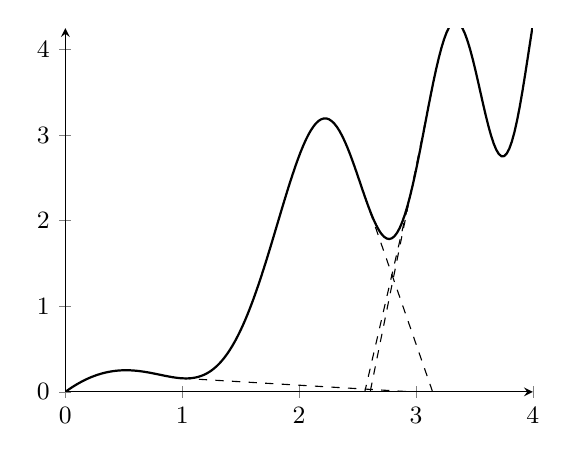
\begin{tikzpicture}
\begin{axis}[width=.62\linewidth,height=6.2cm,xmin=0,xmax=4,ymin=0,ymax=4.25,axis lines=left,tick label style={font=\small}]
\addplot[thick,domain=0:4,samples=180] {x-sin(deg(x^2))};
% Newton tangent segments for the x0=1 sequence
\addplot[dashed,domain=1:2.97] {1-sin(deg(1)) + (1-2*cos(deg(1)))*(x-1)};
\addplot[dashed,domain=2.56:2.97] {2.97-sin(deg(2.97^2)) + (1-2*2.97*cos(deg(2.97^2)))*(x-2.97)};
\addplot[dashed,domain=2.56:3.14] {2.56-sin(deg(2.56^2)) + (1-2*2.56*cos(deg(2.56^2)))*(x-2.56)};
\addplot[dashed,domain=2.61:3.14] {3.14-sin(deg(3.14^2)) + (1-2*3.14*cos(deg(3.14^2)))*(x-3.14)};
\end{axis}
\end{tikzpicture}
\caption{Newton 法求解方程 $x-\sin x^2=0$，初值选取 $x_0=1$ 的迭代序列}
\label{fig:newton-cycle}
\end{figure}

\subsection{弦割法}

Newton 法要求函数的导数值，导数的计算不仅会增加额外的计算量，而且在很多情况下严格计算变得困难甚至无法计算。一个自然的想法是，既然每次迭代需要计算一次导数值且只使用一次，那么我们是否能不严格计算导数而是给出导数的某个近似，从而减小计算复杂度呢？作为最简单的近似，导数可以由两个迭代步的差分给出：
\[
f'(x_k)\approx\frac{f(x_k)-f(x_{k-1})}{x_k-x_{k-1}}.
\]
用其来替代 Newton 法中的导数，我们便得到了迭代公式
\begin{equation}
\begin{aligned}
x_{k+1}&=x_k-\frac{f(x_k)}{f(x_k)-f(x_{k-1})}(x_k-x_{k-1})\\
&=\frac{x_{k-1}f(x_k)-x_kf(x_{k-1})}{f(x_k)-f(x_{k-1})},
\end{aligned}
\tag{2.4.1}
\end{equation}
这便是弦割法。可以证明，如果函数零点处导数
\[
f'(x_0)\ne0,
\]
弦割法的收敛阶是 $p=(\sqrt5+1)/2\approx1.618$。这个收敛速度是超线性的，介于 Newton 法和二分法之间。另外，其对迭代初值的要求和每步的计算消耗也介于两者之间。当然，与 Newton 法一样，弦割法同样不能保证一定收敛。

而弦割法的名称来自其几何对应：如图 2.5 所示，(2.4.1) 式相当于过曲线 $f(x)$ 上两点 $(x_k,f(x_k))$ 和 $(x_{k-1},f(x_{k-1}))$ 作直线，与 $x$ 轴相交于 $(x_{k+1},0)$ 点。

\begin{figure}[htbp]
\centering
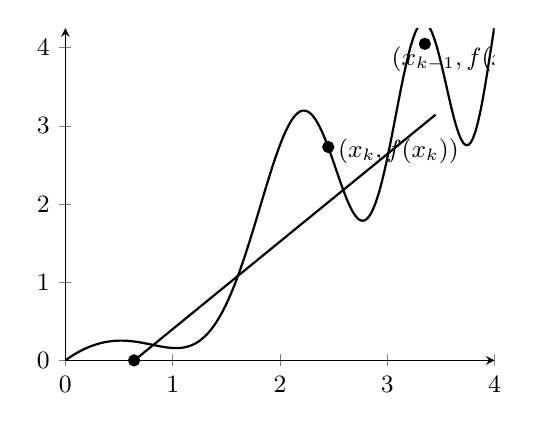
\begin{tikzpicture}
\begin{axis}[width=.58\linewidth,height=5.8cm,xmin=0,xmax=4,ymin=0,ymax=4.25,axis lines=left,tick label style={font=\small}]
\addplot[thick,domain=0:4,samples=180] {x-sin(deg(x^2))};
\addplot[thick,domain=.45:3.45] {1.12*x-0.72};
\addplot[only marks,mark=*,mark size=2pt] coordinates {(2.45,2.73) (3.35,4.05) (.64,0)};
\node[anchor=west,font=\small] at (axis cs:2.45,2.68) {$(x_k,f(x_k))$};
\node[anchor=west,font=\small] at (axis cs:2.95,3.85) {$(x_{k-1},f(x_{k-1}))$};
\node[anchor=north,font=\small] at (axis cs:.64,.05) {$(x_{k+1},f(x_{k+1}))$};
\end{axis}
\end{tikzpicture}
\caption{弦割法示意图}
\label{fig:secant}
\end{figure}

弦割法存在一个确保收敛的修正版本：从一正一负两个迭代初值出发，在随后的迭代中始终取历史迭代序列中具有最大的负值和最小的正值的两个点来计算下一步，这看上去就像是一个改善版本的二分法，通常被称为试位法。但是，实践中会发现，在迭代数步以后，往往会出现其中一个点永远不再被更新的情况，进而收敛阶退化成线性收敛。具体的收敛速度将会依赖于初值的选取和函数的性质，有时还不如二分法来得快。

\subsection{Dekker 算法}

从上面的讨论中我们得知：二分法能保证一定收敛，但不够快；弦割法如果能收敛则是超线性收敛，但却不一定能收敛。我们能不能将两种方法结合起来，在合适的时候选取弦割法或二分法呢？

对这个问题的第一个尝试是 Dekker 做出的。\footnote{Dekker T J. Finding a zero by means of successive linear interpolation // Dejon B, Henrici P. \textit{Constructive Aspects of the Fundamental Theorem of Algebra}. Wiley-Interscience, 1969.}


\begin{algorithmBox}[算法 2.7\quad Dekker 算法]
\begin{lstlisting}[style=bellacode]
function Dekker(func,a,b,eps)
    fa = func(a)
    fb = func(b)
    if(fa*fb > 0) stop "bad section"

    bOld = a
    fbOld = fa
    while(abs(b-a)>eps && fb!=0)
        if(abs(fb) > abs(fa))
            swap(a,b)
            swap(fa,fb)
        end
        m = (a+b)/2
        if(fb != fbOld)
            s = (b*fbOld - bOld*fb)/(fbOld - fb)
        else
            s = m
        end
        bOld = b
        fbOld = fb
        if(m<s<bOld || bOld<s<m)
            b = s
        else
            b = m
        end
        fb = func(b)
        if(fbOld*fb < 0)
            a = bOld
            fa = fbOld
        end
    end
    return b
end
\end{lstlisting}
\end{algorithmBox}

这段代码略微有些长，但其主要思想还是很朴素的。迭代过程中维护两组序列 $\{a_k\}$ 和 $\{b_k\}$，确保每一步时它们分别在函数零点的两端：$f(a_k)f(b_k)\le0$，并且 $b_k$ 相对 $a_k$ 而言是更好的近似：$|f(b_k)|\le|f(a_k)|$；迭代时优先利用 $b_{k-1}$ 和 $b_k$ 试用弦割法，如果弦割法给出的新位置没有落在中点 $(a_k+b_k)/2$ 与 $b_k$ 之间，或者新位置函数值的绝对值并没有下降，则采用二分法。在更新序列时始终将函数值绝对值最小的那个点作为新的 $b_{k+1}$，然后将与其函数值反号的点作为 $a_{k+1}$，以保证收敛性。

Dekker 算法可以有效地改善试位法收敛阶退化的困难：用于弦割法的是相邻两个最优迭代点，而非零点左右两点。对于多数函数，在给出一正一负两个边界后，该算法都能够以超线性的收敛阶稳定地收敛到一个零点上。

\subsection{Brent 算法}

我们之前提到过，Newton 法和弦割法超线性收敛的前提条件都是函数在零点处导数不为零，换言之该零点是一阶零点。对于一些表现足够奇异的函数，尽管弦割法、Newton 法等方法都能确保收敛，但其收敛速度会远远不如二分法。例如，考虑函数
\begin{equation}
f(x)=\begin{cases}
x\exp\left(-\dfrac1{x^2}\right),&x\ne0,\\[0.8ex]
0,&x=0.
\end{cases}
\tag{2.4.2}
\end{equation}
该函数在全空间单调、无穷阶可微，显然前面介绍过的任意算法都一定能收敛到其零点 $x^*=0$。但注意到其零点处任意阶导数均为零，可以证明弦割法和 Newton 法都是弱线性收敛。Dekker 算法同样也会在每个迭代步都选择弦割法，从而无法摆脱弱线性收敛性。

Brent 在 Dekker 算法的基础上提出了额外的判据来避免这个问题。\footnote{Brent R P. Chapter 4: An algorithm with guaranteed convergence for finding a zero of a function // Cliffs E. \textit{Algorithms for Minimization without Derivatives}. Prentice-Hall, 1973.}此外，他使用逆二次插值（inverse quadratic interpolation）来替代弦割法所用的线性插值，以提高收敛速度。

具体而言，当我们有了三个坐标点 $\{x_1,x_2,x_3\}$ 以及其上的函数值 $\{f(x_1),f(x_2),f(x_3)\}$，若三处函数值两两之间不相等，可以构造如下二次多项式以拟合 $x=f^{-1}(y)$：
\begin{equation}
P(y)=\sum_{i=1}^{3}x_i\prod_{j\ne i}\frac{y-f(x_j)}{f(x_i)-f(x_j)}.
\tag{2.4.3}
\end{equation}
容易检验，这个二次函数满足 $P[f(x_i)]=x_i$。不难发现，这个多项式可以更一般地推广至 $n$ 次多项式拟合 $n+1$ 组数据的情形，也就回到了我们前面介绍过的 Lagrange 插值多项式。在这里，借助插值多项式我们可以近似给出 $f(x)=y=0$ 处的坐标值
\begin{equation}
x=\sum_{i=1}^{3}x_i\prod_{j\ne i}\frac{-f(x_j)}{f(x_i)-f(x_j)}.
\tag{2.4.4}
\end{equation}
经 Brent 改善后的算法被称为 Brent--Dekker 算法。

\begin{algorithmBox}[算法 2.8\quad Brent--Dekker 算法]
\begin{lstlisting}[style=bellacode]
function BrentDekker(a,b,func,eps)
    fa = func(a)
    fb = func(b)
    if(fa*fb > 0) stop "bad section"
    if(abs(fb) > abs(fa))
        swap(a,b)
        swap(fa,fb)
    end
    c = a
    fc = fa
    mflag = true
    while( fb != 0 && abs(b-a)>eps)
        if(fa != fc && fb != fc)
            s = a*fb*fc/(fa-fb)/(fa-fc) +
                b*fa*fc/(fb-fa)/(fb-fc) +
                c*fa*fb/(fc-fa)/(fc-fb)
        else
            s = b-fb*(b-a)/(fb-fa)
        end
        if( s is not between (3a+b)/4 and b ||
            ( mflag && abs(s-b) >= abs(b-c)/2) ||
            (!mflag && abs(s-b) >= abs(c-d)/2) ||
            ( mflag && abs(b-c) < eps) ||
            (!mflag && abs(c-d) < eps) )
            s = (a+b)/2
            mflag = true
        else
            mflag = false
        end
        fs = func(s)
        d = c
        c = b
        if(fa*fs < 0)
            b = s
            fb = fs
        else
            a = s
            fa = fs
        end
        if(abs(fa) < abs(fb))
            swap(a,b)
            swap(fa,fb)
        end
    end
    return b
end
\end{lstlisting}
\end{algorithmBox}
\jiaokan{算法 2.8 原代码第 6、7 行将交换操作误拼为 \texttt{swtich}，结合算法 2.7 中同一操作及算法语义，应为 \texttt{swap}；此外原代码在 \texttt{return b} 后缺少与函数定义配对的 \texttt{end}，本版补齐。}

数学软件 MATLAB 中内置的求解函数零点的子程序 \texttt{fzero} 所使用的其实就是 Brent--Dekker 算法。

\begin{exerciseBox}[练习 2.3]
Kepler 方程
\[
M=E-e\sin E
\]
给出了平方反比力场下质点的运动方程。其中平近点角 $M$ 正比于时间，$e$ 为轨道偏心率，偏近点角 $E$ 可以用于计算质点的位置：
\[
\begin{cases}
x=a(\cos E-e),\\
y=a\sqrt{1-e^2}\sin E.
\end{cases}
\]
对于 $e>1$ 的双曲线轨道，通常改用实的双曲偏近点角 $H$，相应的实形式为 $M_h=e\sinh H-H$；若从椭圆方程作复解析延拓，则可令 $E=iH$ 并相应变换平近点角。\jiaokan{原文称“对于 $e>1$ 的双曲线轨道，$M$ 和 $E$ 均应取作虚数”。标准天体力学处理中通常使用实的双曲偏近点角 $H$ 和双曲 Kepler 方程 $M_h=e\sinh H-H$；把 $E$ 取为虚数可理解为从椭圆方程作解析延拓，但不宜表述为物理量“应取作虚数”。}试设计和选用合适的算法，对于任给的 $M$ 和 $e$ 值，都能准确求解出相应的偏近点角并计算质点的位置。
\end{exerciseBox}

\section{平衡点：数值最优化}

上一节所讨论的数值求根问题，还与另一类重要的力学问题直接相关，即求解质点的平衡位置。我们知道，物体在平衡点处的受力
\[
F(x)=0.
\]
而由于力等于势能的负导数，这也对应于势场的极值点：
\[
V'(x)=0.
\]
因此，只要我们能够求得势函数的导数，就能通过应用上一节所学的数值求根方法来找到其极值点，从而求得质点的平衡位置。

但是，这里我们提出一个问题：能否绕开求导，直接求解势函数的极值？答案是肯定的，这一节中，我们来讨论这一类的数值最优化问题。

\subsection{黄金分割法}

黄金分割法是求解数值最优化问题最著名的方法之一，又称华罗庚法、618 法、优选法等，有些读者可能在高中时期就听说过。20 世纪 60--70 年代，华罗庚曾带队在全国各地推广该方法，产生了广泛的影响。

黄金分割法最适用的对象是给定区间 $[a,b]$ 上的单峰函数 $f(x)$。对于求极大值的情形，单峰函数定义为满足如下条件的函数：$\exists x^*\in[a,b]$，使得 $f(x)$ 在 $[a,x^*]$ 上单调递增，而在 $[x^*,b]$ 上单调递减。

二分法无法直接应用于求极值的问题。任取 $x\in[a,b]$ 并求得 $f(a),f(x),f(b)$ 的值，若有 $f(a)<f(x)<f(b)$ 或 $f(a)>f(x)>f(b)$，可以确定函数极大值位于子区间 $[x,b]$ 或者 $[a,x]$ 内，但对于其他情况，我们便无法给出任何判断。从而，我们需要三分区间。

如图 2.6 所示，假使我们在区间中取两个点 $a<x_1<x_2<b$（注意 $x_1$ 和 $x_2$ 未必是三等分点）。如果有 $f(x_1)>f(x_2)$，可以推断在区间 $[x_2,b]$ 中函数 $f(x)$ 一定是单调递减的，从而函数极值点位于区间 $[a,x_2]$ 中，同时容易判断函数在这个区间内依旧是单峰函数，因而可以将这个操作再次应用在子区间 $[a,x_2]$ 上。若 $f(x_1)<f(x_2)$，则反过来，把区间缩小到 $[x_1,b]$ 即可。如果在机器精度范围内碰巧有 $f(x_1)=f(x_2)$，那就能把搜索范围缩小到 $[x_1,x_2]$。

\begin{figure}[htbp]
\centering
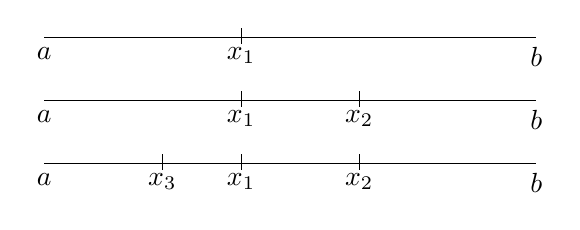
\begin{tikzpicture}[x=1.25cm,y=.8cm]
  \draw (0,2.2)--(5,2.2); \node[below] at (0,2.2){$a$}; \node[below] at (2.0,2.2){$x_1$}; \node[below] at (5,2.2){$b$}; \draw (2.0,2.1)--(2.0,2.35);
  \draw (0,1.2)--(5,1.2); \node[below] at (0,1.2){$a$}; \node[below] at (2.0,1.2){$x_1$}; \node[below] at (3.2,1.2){$x_2$}; \node[below] at (5,1.2){$b$}; \draw (2,1.1)--(2,1.35); \draw (3.2,1.1)--(3.2,1.35);
  \draw (0,.2)--(5,.2); \node[below] at (0,.2){$a$}; \node[below] at (1.2,.2){$x_3$}; \node[below] at (2.0,.2){$x_1$}; \node[below] at (3.2,.2){$x_2$}; \node[below] at (5,.2){$b$}; \draw (1.2,.1)--(1.2,.35); \draw (2,.1)--(2,.35); \draw (3.2,.1)--(3.2,.35);
\end{tikzpicture}
\caption{黄金分割法寻找单峰函数极大值的搜寻步骤}
\label{fig:golden-search}
\end{figure}

得到一个子区间后，原则上又得在该子区间内再取两个点，进行下一步判断以便不断缩小搜索范围。为了方便讨论，我们不妨设取的子区间是 $[a,x_2]$。值得注意的是，在上一步中已经计算了子区间 $[a,x_2]$ 中的一个分点 $x_1$ 处的函数值了，因此可以直接使用，我们只需要再补一个分点 $x_3$ 即可。如果我们期待每一步迭代过程的区间划分都是相似且左右对称的，则有
\[
\tau=\frac{x_2-a}{b-a}=\frac{x_1-a}{x_2-a}>0,
\]
且
\[
x_2-a=b-x_1.
\]
从上面两式可以解出比值
\[
\tau=\frac{\sqrt5-1}{2}\approx0.618,
\]
正是著名的黄金分割比，同样也是算法名称的来源。整理一下上述讨论过程，便可以写出黄金分割法的算法。

在执行 $n$ 步后，以上算法能够返回一个精度为 $O(\tau^n)$ 的极值点位置，从而这是一个线性收敛的迭代算法。注意，在算法中我们并没有对 $f(x_2)=f(x_1)$ 的情形做特殊处理，这是因为有数值计算误差的存在，此类事件发生的概率实在太低。

\begin{algorithmBox}[算法 2.9\quad 黄金分割法]
\begin{lstlisting}[style=bellacode]
function GoldenSection(func,a,b,eps)
    tau = (sqrt(5)-1)/2
    x2 = a + (b-a)*tau
    x1 = a + b - x2
    fa = func(x2)
    fb = func(x1)
    while (b-a > eps)
        if (fb < fa)
            a = x1
            x1 = x2
            fb = fa
            x2 = a + (b-a)*tau
            fa = func(x2)
        else
            b = x2
            x2 = x1
            fa = fb
            x1 = b - (b-a)*tau
            fb = func(x1)
        end
    end
    if(fb > fa)
        x = x1
    else
        x = x2
    end
    return x
end
\end{lstlisting}
\end{algorithmBox}

值得指出的是，对于给定步数 $n$，可以通过精心设计每步的位置来得到一个优于 $n$ 步黄金分割法的区间分割方法，即所谓 Fibonacci 法，但是其精度会低于 $n+1$ 步黄金分割法，从而通常没人会为了效率的这个微小提高而去使用一个设计上相对复杂很多的算法。但对此感兴趣的读者可以阅读参考书 [7]。

\subsection{抛物线法}

除去与数值求根的二分法类似的黄金分割法外，数值求根的弦割法在求解函数极值方面同样也有类似的对应方法，即抛物线法。抛物线法的思路非常朴素，既然通过两个点就能画一条直线寻求零点，那么通过三个点构造一条抛物线可以用来寻找函数的极值点。具体来说，设有三个点 $x_1,x_2,x_3$ 以及其对应的函数值 $f_1,f_2,f_3$，我们便能借助二次函数 $g(x)=a(x-x_0)^2+b$ 求解方程组
\[
g(x_i)=f_i\qquad(i=1,2,3),
\]
消掉 $a$ 和 $b$ 来得到 $x_0$ 的值：
\[
x_0=\frac12\frac{f_1(x_2^2-x_3^2)+f_2(x_3^2-x_1^2)+f_3(x_1^2-x_2^2)}
{f_1(x_2-x_3)+f_2(x_3-x_1)+f_3(x_1-x_2)}.
\]
$x_0$ 可以作为函数 $f(x)$ 在给定区间上极值的一个粗略近似。下一步，用 $\{x_0,x_1,x_2\}$ 作为新的 $\{x_1,x_2,x_3\}$，在一个更小的区间里重复以上操作，直到极值被限制在一个所要求的某一个精度范围内。抛物线法的算法如下。

\begin{algorithmBox}[算法 2.10\quad 抛物线法]
\begin{lstlisting}[style=bellacode]
function Parabola(func,x1,x2,x3,eps)
    f1 = func(x1)
    f2 = func(x2)
    f3 = func(x3)
    while(abs(x1-x2)>eps && abs(x1-x3)>eps)
        x0 = (f1*(x2^2-x3^2)+f2*(x3^2-x1^2)+f3*(x1^2-x2^2))
             /(f1*(x2-x3)+f2*(x3-x1)+f3*(x1-x2))/2
        f0 = func(x0)
        x3 = x2
        f3 = f2
        x2 = x1
        f2 = f1
        x1 = x0
        f1 = f0
    end
    return x0, f0
end
\end{lstlisting}
\end{algorithmBox}
\jiaokan{算法 2.10 原代码将数值变量 \texttt{f1}、\texttt{f2}、\texttt{f3} 与括号直接相邻，形式上会被解释为函数调用；根据紧邻正文给出的抛物线顶点公式，此处应为乘法，故补入 \texttt{*}。}

需要注意的是，与函数求根的弦割法类似，抛物线法同样不能保证一定能够收敛到极值点。但在迭代初值足够接近极值点的前提下，抛物线法是超线性收敛的，收敛阶 $p$ 是三次方程 $p^3=p+1$ 的正根，约为 1.32。为了增强抛物线法收敛的稳定性，人们发展了一些初值选取以及迭代替换的策略，但这些策略往往会使得抛物线法退化成线性收敛。因此，本书不对这些策略进行详述，而是建议读者们先使用黄金分割法算几步得到一个充分小的区间，然后再用抛物线法得到一个满足实际需求的精确结果。

\begin{exerciseBox}[练习 2.4]
考虑重力场下对称轴上一点固定的对称陀螺，其章动角 $\theta$ 相当于在等效势场
\[
V_{\mathrm{eff}}(\theta)=\frac{(L_Z-L_3\cos\theta)^2}{2I_1\sin^2\theta}-mgl(1-\cos\theta)
\]
下运动。取 $L_Z/L_3=0.5$，试选用合适的算法，求解陀螺稳定转动的章动角随无量纲参数 $I_1mgl/L_Z^2$ 的变化。
\end{exerciseBox}

% R04 stops at the end of section 2.5, immediately before source section 2.6.

\section{不可积情形：常微分方程的初值问题}

在前面几节中，我们对于一维牛顿方程的两种特殊情形（即作用力仅依赖于时间或位置）做了详细的讨论，引入了计算常规积分和反常积分的数值算法。然而，在很多实际的物理问题中，更一般的情形是外力同时依赖于时间和位置，甚至还依赖于速度，即
\[
m\ddot{x}=F(x,\dot{x},t).
\]
此时，前面所讨论的数值积分方法就无法用于求解这样的质点动力学问题。我们需要设计新的数值算法，才能够求解我们所面临的微分方程。

数学上，这是一个二阶常微分方程，为了方便后续的讨论，我们可以引入动量 $p=m\dot{x}$，将其变成两个一阶方程：
\begin{equation}
\begin{cases}
\dot p=F(x,p,t),\\
\dot x=p/m.
\end{cases}
\tag{2.6.1}
\end{equation}
它们在初始时刻 $t_0$ 的值都是已知的：
\[
x(t_0)=x_0,\qquad p(t_0)=p_0,
\]
而希望求解任意时刻的 $x(t)$ 和 $p(t)$。更一般地，我们可以把 $x(t),p(t)$ 写为一个向量函数 $\bm y(t)$，方程和初条件便可简记为
\begin{equation}
\begin{cases}
\dot{\bm y}(t)=\bm f[\bm y(t),t],\\
\bm y(t_0)=\bm y_0.
\end{cases}
\tag{2.6.2}
\end{equation}
可以看到，方程组左边为待求解函数的一阶导数，而右边对导数没有依赖。我们将这种形式称为一阶常微分方程组的初值问题。实际上，一般的高阶常微分方程都可以等价地变为一阶常微分方程组。

\subsection{存在性与唯一性}

一般而言，面对一个微分方程，数学家们往往关心它的解是否存在且唯一，而物理学家通常只想知道该怎么解，以及解的性质如何。但事情并不总是这样，常微分方程的唯一性定理表述如下：

\begin{keybox}[定理 2.2]
一阶微分方程组初值问题 (2.6.2) 存在唯一连续可微解的条件是，函数 $\bm f(\bm y,t)$ 连续，且对于 $\bm y$ 满足 Lipschitz 条件：
\begin{equation}
\exists L>0,\ \forall \bm y_1,\bm y_2\in\mathbb R^n,\quad
\lVert \bm f(\bm y_1,t)-\bm f(\bm y_2,t)\rVert<L\lVert \bm y_1-\bm y_2\rVert.
\tag{2.6.3}
\end{equation}
\end{keybox}

这里给出一个不满足唯一性定理条件的例子。考虑一维势场
\[
V(x)=-kx^{3/2},\qquad x\ge 0,\ k>0,
\]
质量为 $m$ 的质点在 $t=0$ 时刻被静置于 $x=0$ 处，求解质点的运动。\footnote{这个势场近似对应于一个更为实际的物理模型：考虑套在形如 $y=-kx^{3/2}/g$ 的光滑轨道上的小圆环，求解在重力势场 $V=mgy$ 下小圆环的运动。}这是一个初值问题，由如下微分方程和初始条件给出：
\[
\begin{cases}
x''=\dfrac{3k}{2m}x^{1/2},\\
x|_{t=0}=0,\qquad x'|_{t=0}=0.
\end{cases}
\]
在解析上容易求得，如下函数是问题的解：
\[
x(t)=\left(\frac{k}{8m}\right)^2t^4,\qquad t>0.
\]
然而，注意到这个函数在零点处的函数值、一阶导数以及二阶导数都是零，对于任意 $t_0>0$，如下形式的函数实际上都是方程的解：
\[
x(t)=
\begin{cases}
0,&t<t_0,\\
f(t-t_0),&t\ge t_0.
\end{cases}
\]
也就是说，在给定了初始条件后，牛顿方程无法唯一确定问题的解。从物理上看，质点可以在位置 0 处停留任意时间后再运动，都满足该势场下的运动方程。这源自函数 $x^{1/2}$ 并不满足 Lipschitz 条件：$|x^{1/2}-0^{1/2}|/|x-0|=x^{-1/2}$ 没有上界。在物理上我们可以找出很多理由：现实世界中并不存在这样带有奇异性的势场；由于 $x=0$ 处奇异性的存在，质点模型失效了；由于各种扰动的存在，不需要关心这类问题；等等。无论如何这提醒了我们，在从实际问题中抽象出物理模型和数学表达式时，始终要注意是否提出了一个足够好的问题。

就此，俄罗斯著名数学物理学家 \rusname{Арнольд} 发表过如下评论：\footnote{引自 \rusname{Арнольд} 的《论数学教育》（On teaching mathematics），此处为其中一部分的译文，原文以俄文发表于 \textit{Uspekhi Mat. Nauk}, 1998, 53: 229，英译本见 \textit{Russ. Math. Surv.}, 1998, 53: 229.}
\begin{quote}\small
我还想说的是，相同的唯一性定理也可解释为何在船只停泊码头前的靠岸阶段必须得依靠人工操作：否则的话，如果行进的速度是距离的光滑函数，则整个靠岸的过程将会耗费无穷长的时间。而另外可行的方法则是与码头相撞（当然船与码头之间要有非理想弹性物体以造成缓冲）。顺便说一下，我们必须非常重视这类问题，例如，登陆月球和火星以及空间站的对接，此时唯一性问题都会让我们头痛。
\end{quote}

\subsection{前向 Euler 法}

我们将从最简单的 Euler 法出发来认识求常微分方程初值问题数值解的各种特征。为求解 (2.6.2) 式，我们回顾微分的定义式
\begin{equation}
y'(x)=\lim_{\Delta x\to0}\frac{y(x+\Delta x)-y(x)}{\Delta x},
\tag{2.6.4}
\end{equation}
从而可以写出近似关系
\begin{equation}
f(x,y(x))=y'(x)\approx \frac{y(x+\Delta x)-y(x)}{\Delta x},
\tag{2.6.5}
\end{equation}
即
\[
y(x+\Delta x)\approx y(x)+f(x,y(x))\Delta x.
\]
这个近似等式在 $\Delta x$ 越小的时候越准确。若在待求解函数 $y(x)$ 的定义域 $[x_0,x_n]$ 上顺序选取若干个格点 $\{x_0,x_1,x_2,\ldots,x_n\}$，将这个关系式应用到相邻两个格点上，便可以递推得到 $\{y(x_1),y(x_2),\ldots,y(x_n)\}$ 的近似值。一般将其记作 $\{y_1,y_2,\ldots,y_n\}$。其中，$\Delta x_i\equiv x_i-x_{i-1}$ 称为步长：
\begin{equation}
\begin{aligned}
y_1&=y_0+f(x_0,y_0)\Delta x_1,\\
y_2&=y_1+f(x_1,y_1)\Delta x_2,\\
&\ \vdots\\
y_n&=y_{n-1}+f(x_{n-1},y_{n-1})\Delta x_n.
\end{aligned}
\tag{2.6.6}
\end{equation}
这类方法由于每一步的计算都可以从之前的结果直接得到，故称为显式（explicit）方法。

我们可以用讨论数值积分误差同样的方法，对以上算法的误差进行估计。由 Taylor 展开可知
\[
y(x+\Delta x)=y(x)+y'(x)\Delta x+\frac12y''(\xi)\Delta x^2,
\]
其中 $\xi\in[x,x+\Delta x]$。若假定 $y_n$ 是精确的，则计算 $y_{n+1}$ 所产生的误差 $\delta_{n+1}$ 为
\[
y(x_{n+1})-y_{n+1}=\frac12y''(\xi)\Delta x^2.
\]
我们称这些方法的局部截断误差为二阶，相对于每一步函数值的变化量，其具有一阶精度。\footnote{请注意此处微分方程解法的精度与数值积分中代数精度的区别。}

上面我们假定了 $y_n$ 是精确的，这个假定显然不成立，由 $y_{n-1}$ 来计算它的时候就已经产生误差了。因此我们需要考察误差在每一步计算过程中如何传播和累积。为此，我们联立如下两式：
\[
\begin{cases}
y_{n+1}=y_n+f(x_n,y_n)\Delta x,\\
y(x_{n+1})=y(x_n)+f[x_n,y(x_n)]\Delta x+\dfrac12y''(\xi)\Delta x^2.
\end{cases}
\]
记某一步的总误差量为 $\varepsilon_n\equiv y(x_n)-y_n$，由两式相减可得
\[
\varepsilon_{n+1}\approx \varepsilon_n+\varepsilon_n\,\partial_yf\,\Delta x+\delta_{n+1}.
\]
其中 $\partial_yf$ 一项来自上下两式中 $f$ 的因变量的差异。如果忽略最后的 $\delta_{n+1}$，我们发现误差增大为原来的 $1+\partial_yf\Delta x$ 倍。当然我们需要注意到 $\partial_yf$ 是一个矩阵（其元素形如 $\partial_{y_i}f_j$），我们需要按照将其对角化后的本征值 $E$ 来理解。借助第一章中关于迭代的讨论，可以知道只当这个倍数的绝对值小于 1 的时候，误差才能被控制住而不至于发散。而由于 $\Delta x>0$，那么只要矩阵 $\partial_yf$ 中包含实部大于零的本征值 $E$，误差就一定会在迭代的过程中发散，这实际上代表着系统存在内禀的不稳定性。但是本征值小于零也不一定意味着误差能够被压低，我们还得要求 $|1+E\Delta x|<1$，即本征值必须位于复平面上圆心在 $-1/\Delta x$、半径为 $1/\Delta x$ 的一个圆盘内，这个圆盘被称为算法的收敛域。

来看一个具体的例子。考察方程 $y'=-\lambda y,\lambda>0$。应用前向 Euler 法
\begin{equation}
y_{n+1}=y_n-\lambda y_n\Delta x,
\tag{2.6.7}
\end{equation}
我们可以很容易写出通式
\begin{equation}
y_n=(1-\lambda\Delta x)^n y_0,
\tag{2.6.8}
\end{equation}
而它的解析解是 $y(x)=y(0)e^{-\lambda x}$，表现为收敛到零的行为。我们看到，当 $\lambda$ 超出了算法的收敛域时，方程的数值解本身直接就发散了，与真实解完全不符，更别谈误差控制的问题了。

\subsection{中点 Euler 法}

以上讨论表明，前向 Euler 法在实际应用中碰到了困难，我们需要想办法加以改进。从数值积分的经验中，我们已经知道了用区间的中点作为整个区间平均值的近似会更有优势，因此我们可以写出近似表达式
\begin{equation}
\begin{aligned}
y(x+\Delta x)
&=y(x)+y'(x+\Delta x/2)\Delta x+O(\Delta x^3)\\
&=y(x)+f[x+\Delta x/2,y(x+\Delta x/2)]\Delta x+O(\Delta x^3).
\end{aligned}
\tag{2.6.9}
\end{equation}
这个式子看上去很美，但问题就在于想要计算 $y(x+\Delta x)$ 就得知道 $y(x+\Delta x/2)$ 的值，而要计算 $y(x+\Delta x/2)$ 的值又要提前知道 $y(x+\Delta x/4)$ 的值……因此，我们陷入了无休止的循环。

处理这个麻烦的关键，在于寻找一个近似替代 $y(x+\Delta x/2)$ 的方案。不同的方案选取会产生多种冠以不同人名的算法，这里我们不一一赘述，而只介绍比较常用的一种，即利用近似式 $y(x+\Delta x/2)=[y(x)+y(x+\Delta x)]/2+O(\Delta x^2)$。将这个近似式代入，我们得到的 $f$ 会产生额外 $O(\Delta x^2)$ 的误差，但注意到它后面还乘了 $\Delta x$，这样这一部分对于计算 $y(x+\Delta x)$ 产生的误差值也是 $O(\Delta x^3)$，与后面的那一项同阶，从而不会对算法精度的阶数产生影响。

对以上的讨论略做整理，我们可以得到如下迭代关系式：
\begin{equation}
y_{n+1}=y_n+f\!\left[(x_n+x_{n+1})/2,(y_n+y_{n+1})/2\right]\Delta x_{n+1},
\tag{2.6.10}
\end{equation}
称为中点 Euler 法。以上迭代并不能直接使用，但我们可以利用 2.4 节中讨论过的数值求根算法来从 $y_n$ 中求得 $y_{n+1}$。注意到，我们可以借助前向 Euler 法来得到方程根的一个相当好的估计，因此可以直接使用类似 Newton 法或者弦割法这类超线性收敛的算法来大大降低计算量。类似这种迭代过程中需要数值求根的微分方程算法被称为隐式（implicit）方法。

进一步，我们来看中点 Euler 法的稳定性和收敛域。将 $y_n$ 替换成 $y_n+\varepsilon_n$ 并做一阶展开，有
\[
\varepsilon_{n+1}=\varepsilon_n+(\varepsilon_{n+1}+\varepsilon_n)\,\partial_yf\,\Delta x_{n+1}/2.
\]
移项整理有
\begin{equation}
\varepsilon_{n+1}=\frac{1+\partial_yf\,\Delta x_{n+1}/2}{1-\partial_yf\,\Delta x_{n+1}/2}\,\varepsilon_n.
\tag{2.6.11}
\end{equation}
这里的分子分母应当理解为矩阵乘法与矩阵求逆。我们看到，误差在迭代过程中的演化同样与矩阵 $\partial_yf$ 的本征值 $E$ 息息相关，稳定性要求不等式
\begin{equation}
\left|\frac{1+E\Delta x/2}{1-E\Delta x/2}\right|<1.
\tag{2.6.12}
\end{equation}
这个式子实际上等价于要求 $\operatorname{Re}E<0$，即在左半平面。也就是说只要方程自己没有不稳定性，就一定能够保证误差不会被放大，这类算法被称为 A-稳定的。从而，我们用每一步迭代需要数值求根一次的代价，换取了对误差很好的控制。

\subsection{自适应步长}

在 2.2 节中，我们介绍过数值积分步长自适应调节的办法，类似的思想也可以应用到微分方程的求解上来。

考察某单步算法，步长为 $h$ 时其局部截断误差为 $p_r h^r+O(h^{r+1})$。等步长迭代两步后有误差 $\delta_h\approx2p_rh^r$；退回，再使用 $2h$ 的步长迭代一次，这样的误差约为 $\delta_{2h}\approx p_r(2h)^r$。计算这两种方式所得误差的差值
\begin{equation}
\Delta\approx 2p_rh^r(2^{r-1}-1)\approx(2^{r-1}-1)\delta_h,
\tag{2.6.13}
\end{equation}
便可估算误差 $\delta_h$ 的大小，从而决定应当增大或者减小步长。若步长始终不变，这个操作会增加 50\% 的计算量，但在实际问题中一般而言总是划算的。

\subsection{蛙跳法}

我们看到隐式方法需要额外进行数值求根，读者也许会追问：能不能绕过数值求根，不付出这个额外的计算代价？很幸运，对于物理上所涉及的一些特殊的微分方程组，这的确是可能的。如果我们将一开始的运动方程 (2.6.1) 写成 Hamilton 动力学的形式
\begin{equation}
\begin{cases}
\dot p=-\dfrac{\partial H}{\partial q},\\
\dot q=\dfrac{\partial H}{\partial p},
\end{cases}
\tag{2.6.14}
\end{equation}
并且假定 $\partial_pH$ 不依赖于 $q$，以及 $\partial_qH$ 不依赖于 $p$（这两个条件看上去都很宽松），那么 Hamilton 量会具有形式 $H(p,q,t)=T(p,t)+V(q,t)$。在这个前提下，我们再来考虑之前的中点 Euler 法的最初思想：
\begin{equation}
\begin{cases}
p(t+\Delta t)=p(t)-\dfrac{\partial V}{\partial q}[q(t+\Delta t/2),t+\Delta t/2]\Delta t,\\[1ex]
q(t+\Delta t)=q(t)+\dfrac{\partial T}{\partial p}[p(t+\Delta t/2),t+\Delta t/2]\Delta t.
\end{cases}
\tag{2.6.15}
\end{equation}
我们看到，计算 $p(t+\Delta t)$ 需要已知 $q(t+\Delta t/2)$ 和 $p(t)$ 的值，而依照第二个等式，计算 $q(t+\Delta t/2)$ 需要已知 $p(t)$ 和 $q(t-\Delta t/2)$ 的值……巧妙的是，我们只需要知道初始条件 $p(t_0)$ 和 $q(t_0+\Delta t/2)$，然后保证时间步长 $\Delta t_n$ 是一个常数，就能够顺序地开展后续的迭代演化。

记 $p_n=p(t_n),q_{n+1/2}=q(t_n+\Delta t/2)$，迭代关系写作
\begin{equation}
\begin{cases}
p_n=p_{n-1}-\dfrac{\partial V}{\partial q}[q_{n-1/2},t_{n-1/2}]\Delta t,\\[1ex]
q_{n+1/2}=q_{n-1/2}+\dfrac{\partial T}{\partial p}[p_n,t_n]\Delta t.
\end{cases}
\tag{2.6.16}
\end{equation}
这个显式算法被称为蛙跳法（leapfrog method）。我们不加证明地给出，其具有二阶精度；但作为显式方法，它的稳定域并不是整个左半平面，例如用于简谐振子时稳定性要求 $|\omega\Delta t|<2$。\jiaokan{原文称蛙跳法的“收敛域为左半平面”，这将意味着该显式方法是 A-稳定的，与显式线性多步法的稳定性性质不符。对简谐振子直接分析其放大矩阵可得稳定条件 $|\omega\Delta t|<2$；故本版改正。}当然这个算法还存在着一个启动的问题，毕竟通常的初始条件是给定某一时刻 $p,q$，而不是错开 $\Delta t/2$ 的两个值。这时简单地应用一次前向 Euler 法或者中点 Euler 法即可，这一步的误差并不会对整体的结果影响太大。

\begin{exerciseBox}[练习 2.5]
在进行分子动力学模拟时，人们常用如下格式的 Velocity--Verlet 算法求解 Hamilton 方程：
\begin{equation}
\begin{cases}
p_{n+1/2}=p_n-\dfrac{\partial V}{\partial q}[q_n,t_n]\Delta t/2,\\[1ex]
q_{n+1}=q_n+\dfrac{\partial T}{\partial p}[p_{n+1/2},t_{n+1/2}]\Delta t,\\[1ex]
p_{n+1}=p_{n+1/2}-\dfrac{\partial V}{\partial q}[q_{n+1},t_{n+1}]\Delta t/2.
\end{cases}
\tag{2.6.17}
\end{equation}
试检验该算法具有二阶精度，但不是 A-稳定的。
\end{exerciseBox}
\jiaokan{原文式 (2.6.17) 第三行左端误印为 $p_n$。Velocity--Verlet 的第二个半步更新应得到下一整步的动量，故应为 $p_{n+1}$；本版据算法定义改正。}

\subsection{小结}

至此，我们介绍了最简单的几种求解常微分方程初值问题的数值方法，为了使得本书内容排布相对均匀，我们将在后续章节介绍几种精度更高，也更一般化的算法，比如著名的 Runge--Kutta 算法等。

\section*{大作业：绝热不变量}
\addcontentsline{toc}{section}{大作业：绝热不变量}

对于单自由度非含时的 Hamilton 系统 $H(q,p)$，若其等能线 $H(q,p)=E$ 对应于相空间中的一条简单闭曲线，可以定义所谓的绝热不变量
\begin{equation}
J\equiv\frac{1}{2\pi}\oint p\,dq,
\tag{1}
\end{equation}
其中积分环路即为该等能线。将绝热不变量看作能量的函数，容易检验
\begin{equation}
\frac{dJ}{dE}=\frac{T}{2\pi}=\frac1\omega,
\tag{2}
\end{equation}
其中 $T$ 为系统运动周期，$\omega$ 定义为该系统的角频率。

若在原有的 Hamilton 量中引入一个随时间缓慢变化的参量 $\lambda(t)$，让系统在这个含时 Hamilton 量 $H(q,p;\lambda(t))$ 下演化，经典绝热定理宣称，此时的绝热不变量将近似为与 $\lambda$ 无关的常数：
\begin{equation}
\lim_{d\lambda/dt\to0}\frac{dJ}{d\lambda}=0.
\tag{3}
\end{equation}
此时绝热不变量定义式中的积分沿 $\lambda$ 为常数的轨迹进行。更详尽的讨论请参考理论力学教材。

本题中我们通过研究一个简单力学模型的长期行为来讨论绝热不变量的适用性。如图 2.7 所示，质量为 $m$ 的小圆环 $A$ 套在无穷长竖直光滑直杆上，通过劲度系数为 $k$、原长为 $\ell$ 的轻质弹簧与固定点 $O$ 相连。以 $O$ 为原点，$A$ 点的水平和竖直坐标分别记为 $x,y$，从而，整个系统的 Hamilton 量可以写作
\begin{equation}
H(p_y,y)=\frac{p_y^2}{2m}+\frac12k\left(\sqrt{x^2+y^2}-\ell\right)^2+mgy.
\tag{4}
\end{equation}

\begin{figure}[htbp]
\centering
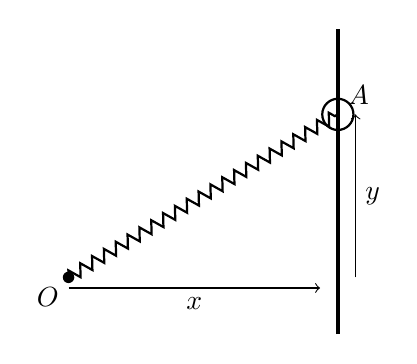
\begin{tikzpicture}[scale=0.9]
  \coordinate (O) at (0,0);
  \coordinate (A) at (3.8,2.3);
  \draw[very thick] (3.8,-0.8)--(3.8,3.5);
  \draw[decorate,decoration={zigzag,segment length=5pt,amplitude=2.2pt},thick] (O)--(A);
  \fill (O) circle (2.3pt) node[below left] {$O$};
  \draw[thick] (A) circle (0.22) node[above right] {$A$};
  \draw[->] (0,-0.15)--(3.55,-0.15) node[midway,below] {$x$};
  \draw[->] (4.05,0)--(4.05,2.3) node[midway,right] {$y$};
\end{tikzpicture}
\caption{关于绝热不变量的简单力学模型}
\label{fig:adiabatic-model}
\end{figure}

\begin{enumerate}
\item 考虑该系统的稳定平衡位置 $y_0$。当 $(x,g)$ 满足什么条件时该系统存在两个稳定平衡位置，什么时候仅存在一个？试解析或数值求解该关系，在 $x$--$g$ 平面上画出这两种情形的分界线。
\item 以速度 $v$ 缓慢地向左移动直杆，那么 $x(t)$ 便构成了慢变参量。取初始时刻 $p_y=0,y=0.1\ell$，以及 $g=0,x(t)=2\ell-vt$。分别对于 $\sqrt{m/k}\,v/\ell=1/4,1/16,1/64,1/256$ 的情形，计算 $x$ 由 $2\ell$ 减小至 0 的过程中系统的相轨，以及绝热不变量 $J$ 随 $x$ 的变化。解释你的结果。
\item 将整个系统放置在一个以频率 $\nu$ 做上下往复运动的电梯里，那么等效重力加速度 $g$ 也可以作为慢变参量。取初始时刻 $p_y=0,y=-2\ell$，以及 $g(t)=2(k\ell/m)\cos 2\pi\nu t,x=0.2\ell$。分别对于 $\sqrt{m/k}\,\nu=1/4,1/16,1/64,1/256$ 的情形，计算 $g$ 从 $2k\ell/m$ 变化为 $-2k\ell/m$ 的过程中系统的相轨，以及绝热不变量 $J$ 随 $g$ 的变化。解释你的结果。
\end{enumerate}

两个参量 $x,g$ 可以同时变化。对于若干个参量自时刻 $t_i$ 经历一系列变化后于时刻 $t_f$ 回到原点的过程，我们可以定义该过程的 Berry 相位。设初末的相空间坐标分别为 $(p_i,q_i)$ 和 $(p_f,q_f)$，Berry 相位定义为
\begin{equation}
\varphi_B=\left[\omega(t_i)\int_{(p_i,q_i)}^{(p_f,q_f)}dt-\int_{t_i}^{t_f}\omega(t)\,dt\right]\bmod 2\pi.
\tag{5}
\end{equation}

\begin{enumerate}[resume]
\item 取初始时刻 $p_y=0,y=-2.1\ell$，以及 $g(t)=2(k\ell/m)\cos2\pi\nu t,x(t)=2\ell\sin2\pi\nu t$。选择充分小的 $\nu$ 以至于 $J$ 近似为常数，检验这样计算得到的 $\varphi_B$ 近似不依赖于 $\nu$。
\item 取初始时刻 $p_y=0,y=0.52\ell$，以及 $g(t)=0.3(k\ell/m)\cos2\pi\nu t,x(t)=0.3\ell\sin2\pi\nu t$。选择充分小的 $\nu$ 以至于 $J$ 近似为常数，检验这样计算得到的 $\varphi_B$ 近似不依赖于 $\nu$。
\end{enumerate}

